%% LaTeX2e class for student theses
%% thesis.tex
%% 
%% Karlsruhe Institute of Technology
%% Institute for Program Structures and Data Organization
%% Chair for Software Design and Quality (SDQ)
%%
%% Dr.-Ing. Erik Burger
%% burger@kit.edu
%%
%% See https://sdqweb.ipd.kit.edu/wiki/Dokumentvorlagen
%%
%% Version 1.3.5, 2020-06-26

%% Available page modes: oneside, twoside
%% Available languages: english, ngerman
%% Available modes: draft, final (see README)
\documentclass[twoside, english]{sdqthesis}

%% ---------------------------------
%% | Information about the thesis  |
%% ---------------------------------

%% Name of the author
\author{Leon Jungemeyer}

%% Title (and possibly subtitle) of the thesis
\title{Rotationally invariant neural networks for homogeneous catalysis}

%% Type of the thesis 
\thesistype{Bachelor's Thesis}

%% Change the institute here, ``IPD'' is default
\myinstitute{Institute of Theoretical Informatics (ITI)}

%% You can put a logo in the ``logos'' directory and include it here
%% instead of the SDQ logo
\grouplogo{aimat-logo}
%% Alternatively, you can disable the group logo
%\nogrouplogo

%% The reviewers are the professors that grade your thesis
\reviewerone{Jun.-Prof. Dr. Pascal Friederich}
\reviewertwo{Prof. Dr. Alexandros Stamatakis}

%% The advisors are PhDs or Postdocs
\advisorone{M.Sc. Chen Zhou}
%% The second advisor can be omitted
% \advisortwo{M.Sc. D}

%% Please enter the start end end time of your thesis
\editingtime{01. December 2020}{31. March 2021}

\settitle

%% --------------------------------
%% | Settings for word separation |
%% --------------------------------

%% Describe separation hints here.
%% For more details, see 
%% http://en.wikibooks.org/wiki/LaTeX/Text_Formatting#Hyphenation
\hyphenation{
% me-ta-mo-del
}

%% --------------------------------
%% | Bibliography                 |
%% --------------------------------

%% Use biber instead of BibTeX, see README
\usepackage[citestyle=numeric,style=numeric,backend=biber]{biblatex}
\addbibresource{thesis.bib}

%% ====================================
%% ====================================
%% ||                                ||
%% || Beginning of the main document ||
%% ||                                ||
%% ====================================
%% ====================================
\begin{document}

%% Set PDF metadata
\setpdf

%% Set the title
\maketitle



%% The Preamble begins here
\frontmatter

%% LaTeX2e class for student theses: Declaration of independent work
%% sections/declaration.tex
%% 
%% Karlsruhe Institute of Technology
%% Institute for Program Structures and Data Organization
%% Chair for Software Design and Quality (SDQ)
%%
%% Dr.-Ing. Erik Burger
%% burger@kit.edu
%%
%% Version 1.3.5, 2020-06-26

\thispagestyle{empty}
\null\vfill
\noindent\hbox to \textwidth{\hrulefill} 
\iflanguage{english}{I declare that I have developed and written the enclosed
thesis completely by myself, and have not used sources or means without
declaration in the text.}%
{Ich versichere wahrheitsgemäß, die Arbeit
selbstständig angefertigt, alle benutzten Hilfsmittel vollständig und genau
angegeben und alles kenntlich gemacht zu haben, was aus Arbeiten anderer
unverändert oder mit Änderungen entnommen wurde.}
 
 
%% ---------------------------------------------
%% | Replace PLACE and DATE with actual values |
%% ---------------------------------------------
\textbf{Karlsruhe, 21.03.2021}
\vspace{1.5cm}

\dotfill\hspace*{8.0cm}\\
\hspace*{2cm}(\theauthor) 
\cleardoublepage

\setcounter{page}{1}
\pagenumbering{roman}

%% ----------------
%% |   Abstract   |
%% ----------------
 
%% For theses written in English, an abstract both in English
%% and German is mandatory.
%%
%% For theses written in German, a German abstract is sufficient.
%%
%% The text is included from the following files:
%% - sections/abstract

\includeabstract

%% ------------------------
%% |   Table of Contents  |
%% ------------------------
\tableofcontents

\listoffigures
%\listoftables

%% -----------------
%% |   Main part   |
%% -----------------

\mainmatter

%% LaTeX2e class for student theses
%% sections/content.tex
%% 
%% Karlsruhe Institute of Technology
%% Institute for Program Structures and Data Organization
%% Chair for Software Design and Quality (SDQ)
%%
%% Dr.-Ing. Erik Burger
%% burger@kit.edu
%%
%% Version 1.3.5, 2020-06-26

\chapter{Introduction}
\label{ch:Introduction}

%% -------------------
%% | Example content |
%% -------------------

Catalysts in combination with chemical reactions are used to speed up a reaction by lowering its activation energy. 
Catalysts have an activation energy themselves that needs to be overcome in order to start the reaction, the so called reaction barrier.

The catalyst molecules observed in this thesis are part of Vaska's complex, a chemical compound consisting of a variety of different catalysts all with an iridium atom at their center.
The activation barrier depends on the structure of the catalyst, and varies greatly between different molecules.
Seemingly small changes in the catalysts shape can have a large influence on the catalysts activation barrier [Figure~\ref{fig:struct-diff}].
A rule to guess the activation barrier from the molecules structure cannot easily be found.  
Knowing how to change catalyst molecules in order to lower their activation barrier is a difficult challenge, even to humans.
While the activation barrier can be computed, this process is highly complex and takes a lot of computing power.
This means computing the activation barrier for large datasets of catalysts is currently not feasible.
\\
In this Bachelor's thesis, different approaches to use machine learning to compute the activation barrier of catalyst molecules are explored.
Multiple methods of encoding catalyst molecules into machine-understandable formats are proposed.
Using artificial neural networks, the activation barrier is predicted from the catalysts shape.

After being able to predict the activation barrier with high accuracy, different techniques to explain the 
outputs of the neural network are used.
This helps to better understand booth the network that is usually regarded as a black box, and the feature space.
The explainers used here are simple gradient based methods, and SHAP explainers \cite{NIPS2017_7062}.
This allows for intuition on which parts of the catalyst molecule contribute to the prediction of the activation barrier.
This intuition may be helpful in further chemical analysis of the metal catalyst and can help to give the 
chemist an idea on how an element needs to be changed in oder to lower it's activation barrier.
\\

\begin{figure}
  \centering
  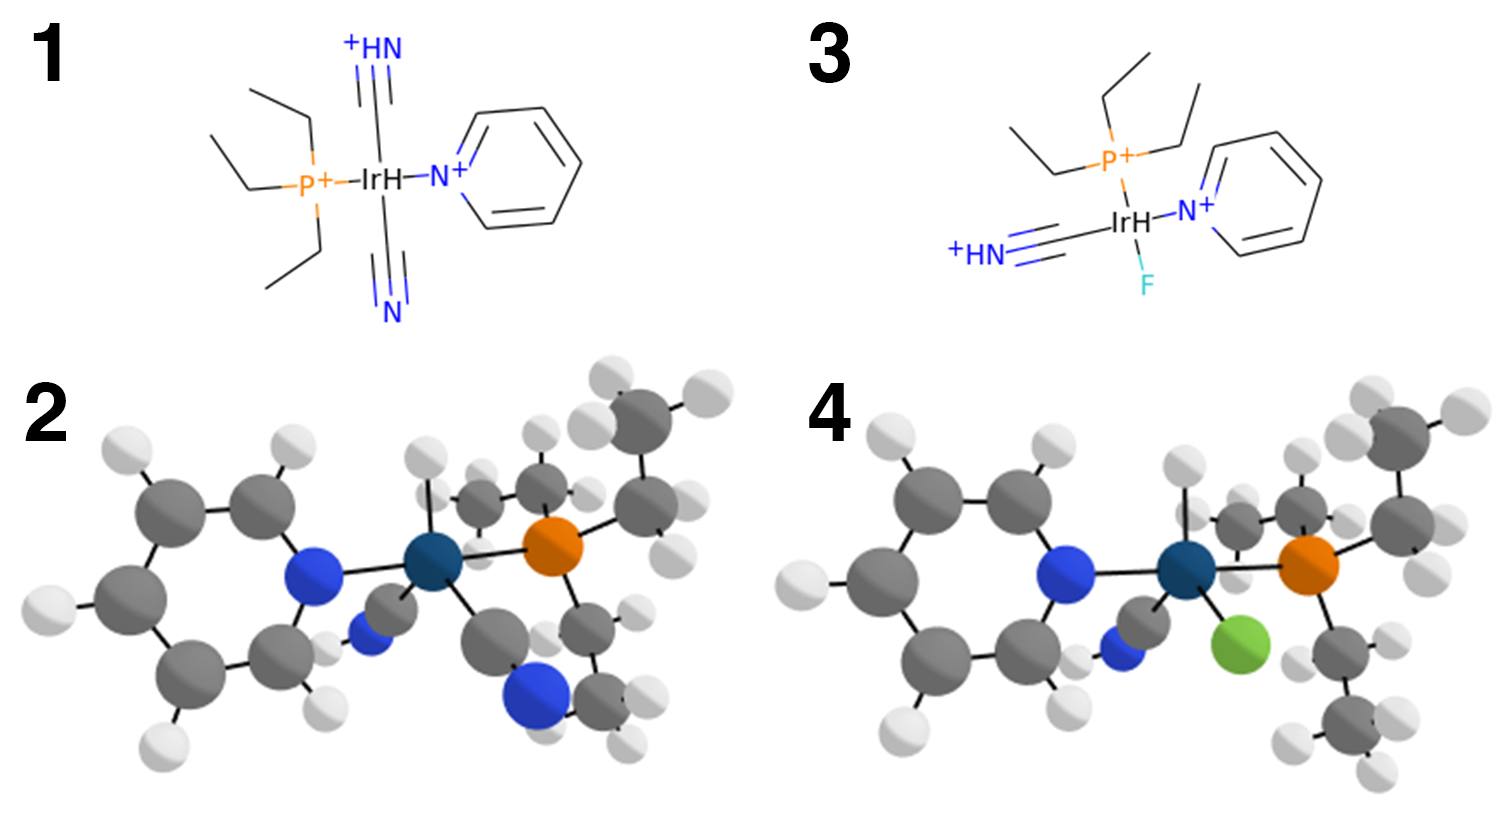
\includegraphics[width=0.8\textwidth]{figures/introduction/elems_intro.png}
  \caption[Example of catalyst molecules]{Two elements with seemingly very similar chemical structures. The chemical structure 1 and it's corresponding 3D structure 2 have an activation barrier of $3.6 kcal/mol$.
  Molecule 3 and it's corresponding 3D structure 4 have an activation barrier of $18.0 kcal/mol$.
  The only difference in the 3D structure of the 2 is the fluorine arm is being replaced by a nitrogen arm.
  The difference is significant considering the distribution of the activation barriers in \ref{fig:barriers}.  }
  \label{fig:struct-diff}
\end{figure}


The metal catalysts in question are constructed by combining different ligands around a central Iridium atom.
As illustrated in Figure~\ref{fig:chemspace}, the central atom has multiple locations that allow different types of ligands to be attached to.  
It enables a quick generation of thousands of different catalyst molecules.
By adding more ligands, the dataset can be increased in size with little effort.
For all catalysts in the dataset the activation barrier, along with other properties, is then computed.
The structure, both chemical and spacial, and the activation barrier is know for every example in the dataset. 
\\
As with many machine learning tasks, feature selection is one of the big challenges in this project.
While there are many universal techniques to extract features from chemical structures, they all have their drawbacks.

In previous works, multiple different techniques are proposed to extract features from a catalyst molecule \cite{friederich_dos}.
These techniques are based on the chemical structure of a molecule, but do not take into account its 3D spacial structure.
This withholds a lot of information to the neural network that might help it to predict more accurately the activation barrier.
The feature extracting methods developed in this bachelor thesis will rely heavily on the 3D structure of the molecule.
The hypothesis is that the 3D structure is playing an important role in the activation barrier, and encoding the 3D structure will enhance regression accuracy.
Additionally encoding 3D structure will allow to learn about the space surrounding the central 
iridium atom to understand the importance of location of the atoms in our molecule.

In order to use feature explainers on the neural network, a reverse mapping from feature space and chemical space needs to be possible.
There currently is no widespread way to encode catalyst molecules that also allows for 
reconstruction of the 3D space and by that an intuition on how the molecule needs to be changed in order ot lower the activation barrier.
Since most chemical feature generators do not specifically focus on catalyst molecules,
but rather provide features for a wide variety of molecules, they generally tend to generate a fully rotational invariant output.
This full rotational invariance means that information about the location of single atoms is often lost or only implicitly encoded in the features.
Therefore a reconstruction of the molecule only from the features is not possible.
The descriptors proposed here allow make use of a catalysts special structure.
This enables a partial reconstruction of the 3D shape of the molecule.
In the future this approach could be used to also encode other properties of the molecule.
\\

The seemingly arbitrary distribution of activation barriers among catalyst molecules  was reason to use neural networks for prediction from the generated features.
Neural networks have become the go-to method for high dimensional regression and classification for their ability to adapt well to complex data.
\\
A limitation of neural networks however is their fixed-size input space.
Therefor a representation of the catalyst needs to be found that encodes molecules into a fixed-size set of features.
These features will then be fed into a neural network for training. 
\\
3D structural encoding comes with its own set of challenges. 
Since a molecules activation barrier does not change depending on its rotation or location in space, 
information about rotation and translation should ideally not be part of the molecules features.
\\
In the case of the metal catalysts, achieving translational invariance is trivial.
Since every catalyst is constructed around exactly one metal atom, the molecule can be centered around this metal atom.

For rotational invariance the problem is more complex.
Every catalyst has a reaction pocket attached to its cental atom.
This reaction pocket has a fixed position.
With the vector from the center of the iridium atom to the center of the reaction pocket, two more degrees of freedom can be removed.
There is no natural way to get rid of the last degree of freedom, rotations around this vector.
%TODO: Figure
Here, 2 different approaches to this last degree of freedom are explored.
The first is using a descriptor that is invariant under rotations around the last degree of freedom.
This removes the need for further normalizations, since all features generated by this descriptor will be invariant.

The second is using data augmentation to teach the neural network about all possible rotations.
This means the molecule is rotated along the last remaining axis of freedom, and and multiple examples of the same molecule at different rotations are used as training examples for the neural network.
This ideally allows the network to abstract away the rotation of a molecule.

After completion of training the networks are able to predict a catalysts activation barrier from its 3D structure.
The main motivation behind encoding the 3D structure is based on the ability to analyse the networks after training.
By analyzing on which features the network is basing its prediction, and translating these features back into 
3D space, we can get an intuition on which parts of the molecule influence its activation barrier.

Additional information about the influence of different species can be gained 
from separately encoding different atom species into their own set of features.

\section{Dataset}

The dataset used for training and testing contains a total of 1947 samples.
Each sample describes the 3D structure of one catalyst molecule, 
containing the position for every atom in that molecule.
Additional information about the molecule was precomputed among the reaction barrier focused on in this work [Figure~\ref{fig:barriers}].
The number of atoms forming one molecule varies between catalysts.
What's consistent is the central iridium atom and the reaction pocket, a single hydrogen atom, attached to the center.
The global position and rotation of the molecule within the dataset is seemingly arbitrary.
Global rotation and location of the element does not influence its activation barrier.
However the local position of atoms in the molecule plays and important role in the activation barrier.

\begin{figure}
  \centering
  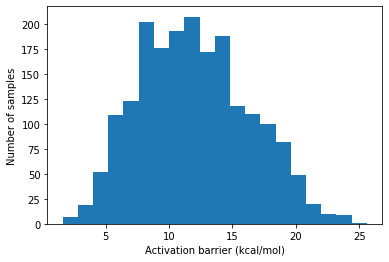
\includegraphics[width=7cm]{figures/introduction/barrier.png}
  \caption[Distribution of activation barriers]{Distribution of the elements activation barrier. The elements have a mean of $11.970 kcal/mol$ and a standart deviation of $4.33 kcal/mol$.}
  \label{fig:barriers}
\end{figure}

The dataset was constructed from a set of ligands.
These ligands are placed around the iridium core in a specific order.
There is a total of 3 ligand groups, with every group being able to attach in a different way to the metal center.
By combining different ligands from these groups, catalysts are created [Figure~\ref{fig:chemspace}].
These chemical structures are known as Vaska's complex.

Due to this combinatorial approach the dataset could later be increased with relatively low effort.
The biggest hurdle to increasing the dataset size is computing the activation barrier.
This computation is highly complex and therefore not feasible for large datasets.
However, generating a larger dataset without computing the activation barrier could still be helpful when using transfer learning approaches to fine tune the network.
This idea is further discussed in [Chapter~\ref{ch:Conclusion}].

\begin{figure}
  \centering
  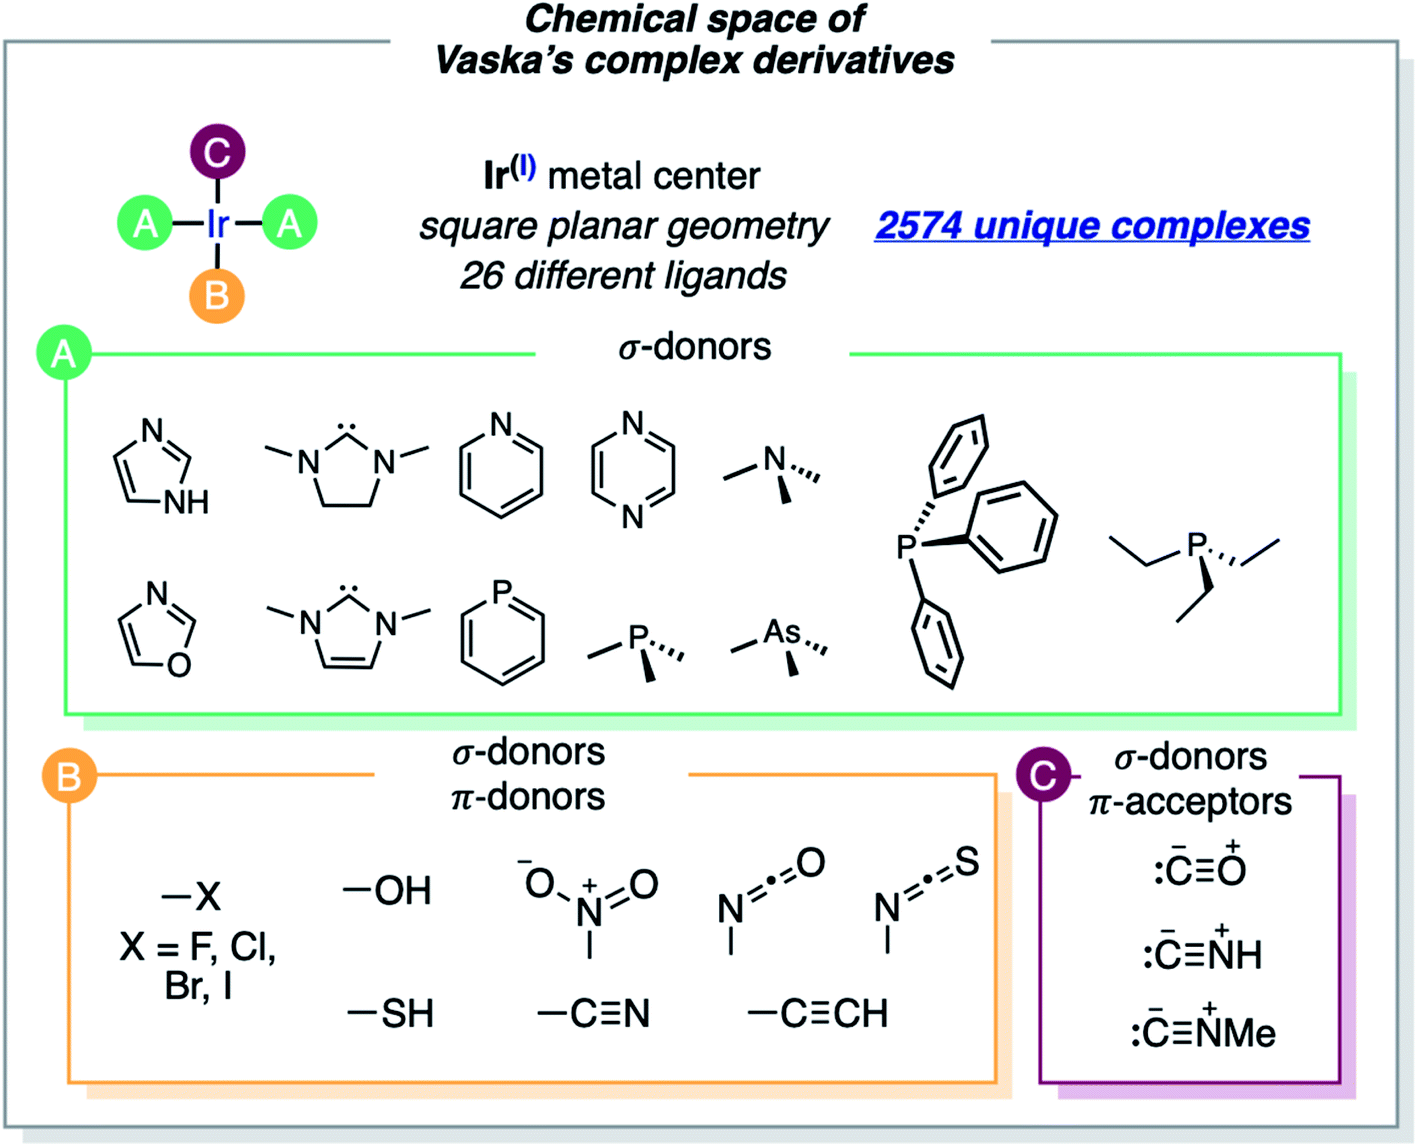
\includegraphics[width=10cm]{figures/introduction/chem-space.png}
  \caption[Vaska's space]{Ligands defining the chemical space associated with Vaska's complex. Reprinted from \cite{friederich_dos}.}
  \label{fig:chemspace}
\end{figure}


\section{Previous research}

In previous approaches different machine learning methods were used to predict the activation barrier of the elements in this dataset.
The features extracted from the elements focused on their atomic properties.
However, the features extracted from the molecule did not take into account the spacial structure of the element.
The elements were instead encoded by creating a graph from the chemical structure.
The elements are then grouped by their distance from the metal center.
For each group of elements, features were computed as sum of pairwise products/differences of their atomic properties(such as electronegativity, atomic number, identity, topology and size) \cite{friederich_dos}.
Note that these features do not contain any information about the 3D location of the atoms.

Using these autocorrelation features, a neural network and other forms of regression were used to predict the activation barrier.
Gaussian processes were able to predict the activation barrier within an error of $<1 kcal/mol$ for a train split of $80\%$.

In a unpublished approach, the autocorrelation features were replaced by a graph structure of the molecule.
On this graph structure, a graph convolutional neural network was trained.
When training on a large fraction of the dataset this network reached accuracies 
beyond what could be achieved using autocorrelation features, reaching accuracies of $<0.5 kcal/mol$ for a training fraction of 90\%.

All of these methods used features independent of the 3D structure of the element.
Other than the obvious disadvantage of withholding information from the element, another disadvantage is the lack of interpretability of results.
While these features succeed at predicting reaction barriers, gaining 
information about what part of the molecule is contributing to the prediction is limited or not possible.

The feature extractors introduced in this thesis aim to solve this problem by extracting features that allow for a
partial reconstruction of the chemical space.
This helps to better understand the origin of a prediction, and might be helpful to better understand 
the underlying elements in a chemical sense.

Feature extraction is a common problem for machine learning methods in chemical spaces.
Multiple approaches have been proposed for general molecule encoding, 
ranging from encoding properties of molecules, such as the Coulomb Matrix encoder encoding electrostatic interaction of atoms \cite{PhysRevLett.108.058301}
to encoding 3D structures of atomic environments \cite{Bart_k_2013}.

3D structural encoders usually create a fully rotational invariant features.
In the case of SOAP proposed by \citeauthor{Bart_k_2013}, this is achieved by encoding information about the interaction of 
different species rather than encoding the 3D space itself.
Fully invariant 3D descriptors have the advantage of being universally applicable for any kind of molecule, since they have no requirements to the element being encoded.
The disadvantages are that, once the features are generated, a transformation back to 3D space is usually not possible.
In many applications, this is not a problem since the generated features are used only for prediction of an elements properties.
In the applications here the features however should later allow to interpret the 3D space surrounding the molecule and ideally give an idea on how the molecule can be changed to alter its properties.

The idea of using a catalysts special structure for this task, and therefore removing some axes of freedom from the feature space, seems to be an unexplored approach.

Since the structure of the catalyst still leaves 1 degree of freedom, the prediction needs to be partly rotationally invariant.
This is a common problem for neural networks even outside of chemistry.
Generally the approaches to solving these problems can be divided into 2 different groups.

The first being feature engineering to generate features from the data that are fully invariant of rotation.
In point clouds approaches include representing the data as angles and distances rather than the points itself \cite{weiler20183d, 8886052}.
Since these features do not change depending on the rotation and translation of the points, the network does not need to 
abstract away the rotational information of the data.
While this method guarantees full rotational invariance, it requires extensive feature engineering.
Additionally, it may increase complexity of the features and in many cases 
goes hand in hand with the loss of some information from the original dataset. 
Restoring the original data is therefore often impossible.
%The EFD feature generator proposed here implements a fully rotationally invariant description by using 
%descriptor that can be normalized for rotation.

A second approach to rotational invariance is data augmentation.
In image recognition data augmentation has already become the go-to method.
Data augmentation removes the need for extensive feature engineering.
Instead, the training data is augmented along all axes of freedom.
In the case of image recognition, this means rotating, scaling, and in some cases deforming the input images.
By that, the dataset will be filled with more examples for every data point, and ideally the model is able to 
abstract away these features. %TODO: Citation needed
In the case of catalyst molecules, each element will be rotated around the remaining axis of freedom.
The different angles will then be fed into to the network for training.
%The SNAP feature generator proposed here produces a partially rotationally invariant output that needs to be augmented along one axis.
%All the augmentation steps are then fed to the networks in order to teach the network to abstract away the different rotations of the catalyst.

\section{Objectives}

As with many machine learning tasks, using the raw data as input to machine learning models is not feasible.
Features are therefore generated from the raw data that can be used to learn from.
The typical workflow for machine learning in chemical fields reflects this approach [\ref{fig:feature-process}].

This work can be grouped into 3 main objectives. 
The first is to find a feature extractor that generates features from a catalyst molecule that ideally rotationally invariant.
The second objective is to train a neural network on these features that predicts the activation barrier.
The goal was to achieve accuracy similar or higher to what \citeauthor{friederich_dos} achieved in \cite{friederich_dos}.
In a final step, using explainers to explain the origins of the networks prediction, an intuition on how a catalyst has 
to be adapted in order to change it's activation barrier is given.


\begin{figure}
  \centering
  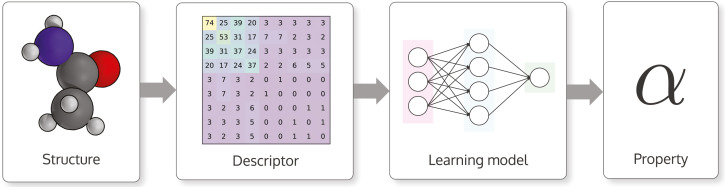
\includegraphics[width=12cm]{figures/introduction/chem-descriptor.jpg}
  \caption[Machine learning in chemistry]{Visualization of feature generation and prediction from the generated features. 
  A fixed size descriptor is generated from the structure. Using machine learning techniques, 
  predictions are made from these features.
  The feature generators proposed here should allow a partial inversion of this process to allow for interpretability of the results.
  Reprinted from \cite{dscribe}.}
  \label{fig:feature-process}
\end{figure}


\subsection{Feature generation}

The features should allow a regressor to make predictions from the 3D shape of the molecules.

Therefor features have to be of fixed length for all elements in the dataset.
The amount of atoms in one element cannot influence the number of features.

Ideally the number of features is as low as possible, helping the model to identify the relevant features better.
The number of features cannot be too small as it should still contain all relevant information.
For interpretability of the results, the features should allow for a partial or full reconstruction of the element they are encoding.
This means, given the features, it should be possible to approximate the general shape of the molecule.

To allow for computational exploration of the encoded space, the features should be continuos.
Small changes in the density space should result in small changes in the 
feature space. 
This means hashing from chemical space to feature space is not viable.

The global location and rotation of the element should not influence the features or have only limited influence on the features.

Two different approaches to feature generation are prosed.
The first is a fully rotationally invariant output using a rotationally invariant contour description.
While the output of this descriptor is fully invariant, it suffers from sampling issues due to the nature of it's encoding.

The second approach to feature generation was using a combination of basis functions to fully describe a local environment around a central atom.
Using a set of coefficients, the density space surrounding the central atom can be approximated.

\subsection{Regression}

The second step is to predict the activation barrier from these features using an artificial neural network.
A reference for prediction accuracy was set by \cite{friederich_dos}.
The networks proposed here achieve higher accuracy's than the best regression methods proposed in \cite{friederich_dos}.

The regression methods performed on features created with method \ref{ch:SNAP} achieve accuracies higher than regression methods on graph convolutions,
the highest accuracy regressors on this dataset to date.

\subsection{Explaining the feature space}
Since the features should be able to allow a inversion back to the 3D space, it's possible to approximate which areas in 3D space are responsible for the prediction.
Using neural networks explainers, in  a last step the regions in 3D space that influence the regression will be analyzed.
This gives an idea on how different atoms in the dataset influence the prediction.
Looking at the gradient of the input with respect to the activation barrier, an intuition on how the catalyst molecule needs to be 
adapted in order to decrease the activation barrier can be given.

Due to the low resolution of the encoder, the information that can be gained is limited.
%% LaTeX2e class for student theses
%% sections/content.tex
%% 
%% Karlsruhe Institute of Technology
%% Institute for Program Structures and Data Organization
%% Chair for Software Design and Quality (SDQ)
%%
%% Dr.-Ing. Erik Burger
%% burger@kit.edu
%%
%% Version 1.3.5, 2020-06-26

\chapter{Feature generation}
\label{ch:features}
%% ==============
Artificial neural networks(ANNs) and other machine learning techniques have strict requirements to their input data.
For ANNs specifically, the input needs to be of fixed size and ideally as low dimensional as possible.
To achieve that, a fixed number of features are extracted from the molecules.
In order to learn, all the data required to predict molecular properties, in this case the activation barrier, should be encoded in the features.
These features can then be used to train a neural network.

Simple encoders extract well know features of molecules such as their mean electro negativity or atomic numbers \cite{LO20181538}.
Approaches by state-of-the-art chemical encoders include using graph convolutions to parse the chemical structure into fixed size features \cite{GNN_ENCODER}.
Others try to encode interaction of different atoms or species of atoms into their features \cite{PhysRevLett.108.058301}.
The feature generators relevant to this project are spacial encoders.

Spacial encoders in chemistry generally focus on describing the interaction of chemical elements within a certain radius, rather 
than the space itself \cite{Bart_k_2013}.
Since global rotation and translation of an element generally does not influence it's chemical properties,
encoders try to produce rotationally invariant representations.
This usually limits the possibilities of reconstructing the input data.
A 3D representation can therefore not easily be computed from the generated features.

The feature generators proposed here have the ability to partly reconstruct the 3D space they are encoding.
In order to retain partial rotational invariance the special structure of the input data is used.
All catalyst molecules in the dataset have a central metal atom and a reaction pocket composed of a hydrogen atom attached to the metal center.
By the centers of these 2 atoms a unique axis is formed.
This axis is used to align the molecules.

The use of this special structure of catalyst molecules to generate partly invariant features seems to be a novel approach.

After alignment, two different approaches to feature generations are explored.
The first method slices the molecule at certain heights.
The slices are then described using a fully rotationally invariant descriptor.

The second approach is to use a combination of different 3D basis functions to encode the space surrounding the central atom.
Since this description is not fully invariant, data augmentation is used along the remaining axes of freedom.

\section{Alignment of catalyst molecules}

Every catalyst molecule $\mathbb{E}$ in the dataset has a central Iridium atom with position $p_{Ir} \in \mathbb{E}$.
The Iridium atom is set to the center, all other atoms are aligned accordingly.

$$ \forall p_i \in \mathbb{E}: p_i' = p_i - p_{Ir}$$

Now that the element is centered, the next step is rotating it.
Every catalysts has a reaction pocket attached to the central metal atom.
This reaction pocket is defined by a single hydrogen atom attached to the central iridium atom.
The goal is to rotate the entire molecule so that the reaction pocket is aligned with the $z$-Axis.
The axis to be aligned is defined by the vector running from the center to the reaction pocket, so

$$ v = \frac{p_{Pocket}'}{\| p_{Pocket}'\| } $$

The vector $v$ is now rotated so that it aligns with the $z$-Axis.
Since this rotation can be defined no matter the elements initial alignment, it effectively removes rotational invariances.
Let $A$ be a plane through the points $(0,0,0), (0,0,1), v$.
The normal $n$ of $A$ is the axis the molecule will be rotated around.

$$
n =\frac{\begin{pmatrix}
  0 &
  0 &
  1
\end{pmatrix}^T \times v}{ \left\| \begin{pmatrix}
  0 &
  0 &
  1
\end{pmatrix}^T \times v \right\| }
$$
Next, the angle $\alpha$ between $v$ and the $z$-Axis on the plane is computed.

$$ 
\alpha = k \cdot \arctantwo \left( 1,  
\begin{pmatrix} 0 &  0 & 1 \end{pmatrix} \cdot v \right),\space k = \left\{\begin{array}{ll} 1, & n \cdot \left( (0,0,1)^T \times v \right) > 0 \\
  -1, & \text{otherwise}\end{array}\right.
$$

A rotation matrix around the normal $n$ can be defined as:
$$
R(\alpha) = I_3 + C \sin(\alpha) + C^2(1 - \cos(\alpha)), C =
\begin{pmatrix}
  0 & -q_0 & q_1 \\
  q_2 & 0 & -q_0\\
  -q_1 & q_0 & 0
\end{pmatrix}
$$


The rotation $R(\alpha)$ can then be applied to all centered atoms in the element.
The aligned and centered molecule can therefor be described as

$$ 
\mathbb{E}^R = \left\{ R(\alpha) (p_i - p_{Ir}) |  p_i \in \mathbb{E} \right\}
$$

The coordinates $p^R_i \in \mathbb{E}^R$ are now rotationally invariant under 2 axes. 
The only degree of freedom left is rotations around the $z$ axis. 

This normalization is repeated for every element in the dataset.

%Since there's no natural way to align the elements around $z$, different approaches will be used.
%In a first attempt, features are generated using a descriptor that is fully invariant under rotations around $z$.
%The second descriptor is using data augmentation to teach the network about possible rotations of the molecule.





\section{Fourier descriptors for invariant feature generation}

The first attempt at feature generation was using a fully rotational invariant feature descriptor.
The method used is an Elliptic Fourier Descriptor (EFD).
Elliptic fourier descriptors approximate a 2D contour with a set of coefficients.
The higher the order of the descriptor, the better a contour can be approximated.

To be able to describe a 3D object using fourier contour descriptors the object is sliced at different $z$ heights.
For each slice, the contour is described using an EFD.
This generates a fully rotationally invariant description.
Since EFDs allow to approximate a contour with just a few coefficients, the generated features
are also low dimensional.
This feature generator will be referred to as layered elliptic fourier descriptor(LEFD).

\subsection{Slicing}
\begin{figure} [h]
  \centering
  \includegraphics[width=0.5\textwidth]{figures/fourier/slice3D.png} % for .pdf files etc use \includegraphics{test.pdf}
  \caption[Slicing a molecule]{A molecule is sliced by a plane. Every slice is taken at a different $z$ height.}
  \label{fig:slice3D}
\end{figure}

Along the $z$-axis, starting from $z_{start}$ to $z_{end}$, the molecule is sliced in a distance of $z_{height}$.
$z_{start}, z_{end}, z_{height}$ are tuning parameters.
Here, $z_{start}, z_{end}$ are chosen so that all molecules from the dataset fully fit into the boundaries.

A slice is computed by getting the radius of every atom $i$ in the molecule at the slice height $z$ Figure~\ref{fig:slice3D}.

$$ r_i(z) =\left\{\begin{array}{ll} \sqrt{R_i^2 - (z - p_i^R[2])^2} &, | z - p_i^R[2] |  < R_i\\
  0 &, \text{otherwise}\end{array}\right.
$$ %TODO: Der Betrag ist immer > 0 ???

$R_i$ is the Van-der-Waals radius of element $i$, $p_i[2]$ is the $z$ component of the location vector.
The slice is now constructed by drawing a circle with radius $r_i(z)$ around the $x,y$ coordinates for each atom for each slice Figure~\ref{fig:slice}.

\begin{figure} [h]
  \centering
  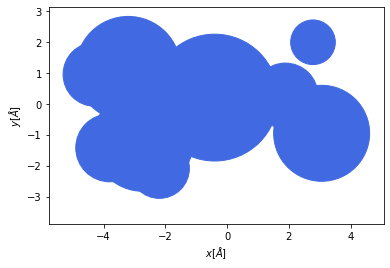
\includegraphics[width=0.5\textwidth]{figures/fourier/slice-iso.png} % for .pdf files etc use \includegraphics{test.pdf}
  \caption[Visualization of a slice with isolates]{A slice with isolates.}
  \label{fig:slice}
\end{figure}

The slice consists of a set of circles.
These circles can be partially or fully intersecting. 

To describe the contour, a fourier contour descriptor is used.
This contour descriptor allows to easily ignore rotation of the contour and generate invariant low-dimensional features from the shape.
However, it can only work on a closed contour, so isolate islands of circles that don't intersect have to be dealt with separately.
For simplicity, islands will be ignored by the contour descriptor.
To identify islands and one continuos subset of circles, for each slice a graph is constructed.
For every atom with radius $>0$ we create a node.
For every atom that intersects with another we create an edge between these two nodes.
Now the \texttt{Largest Connected Component}, so the connected subgraph with the most nodes, is computed.
This gives us the most atoms forming a continuously connected shape in the current slice.
In the next steps we will only use this subset of circles to describe the contour.
%TODO: Not perfect, but good enough?
\paragraph{Finding the contour}

From the set of intersecting circles, the contour needs to be extracted. 
Since the contour points are computed just from radius and position information, and are not rendered onto a 2D pixel grid, standard contour finding algorithms can not be used.
Instead, knowledge about the general shape is used to compute the contour. 

The contour is computed using \autoref{alg:CircleSetContour}.

First, the point "furthest to the right", so with the largest $x$-Value is found. 
Since the point with the highest $x$-Value in any circle is always at angle 0, we set the initial angle $\alpha$ and rotation vector $\vec{p}$ accordingly.
From the circle containing that point, the contour is followed from that point counter-clockwise until the first intersection with another circle is found.
To the list of contour sections, we add the current contour section from angle $0$ to the angle of intersection.

Now, the contour of this circle is followed again until it intersects another. This is repeated until the starting circle is reached again.

Once the starting circle is reached, the last remaining contour part of the starting circle needs to be added to the list of contour sections Figure~\ref{fig:circlesetcontour}.

From the ordered list of contour sections, the contour points can easily be computed.
Since each contour section consist of a radius $r$, location $(x,y)$, and start- and end angle $\alpha_{start}, \alpha_{end}$, the coordinates of the contour points can simply be computed using $x_c = \cos(\alpha_c) \cdot r + x$ and  $y_c = \sin(\alpha_c) \cdot r + y$ 
for $\alpha_c = \alpha_{start} + i \cdot \Delta, \alpha_c \leq \alpha_{end}, i \in \mathbb{N}_0$.

$\Delta$ is a tuning parameter that specifies the resolution of the contour.

This process of going along the outside ignores all "holes" in the shape, so only the outermost contour will be part of the final result. 
This is beneficial since EFDs only allow for the encoding of a single closed contour.

\begin{figure}[!htb]
  \minipage{0.32\textwidth}
    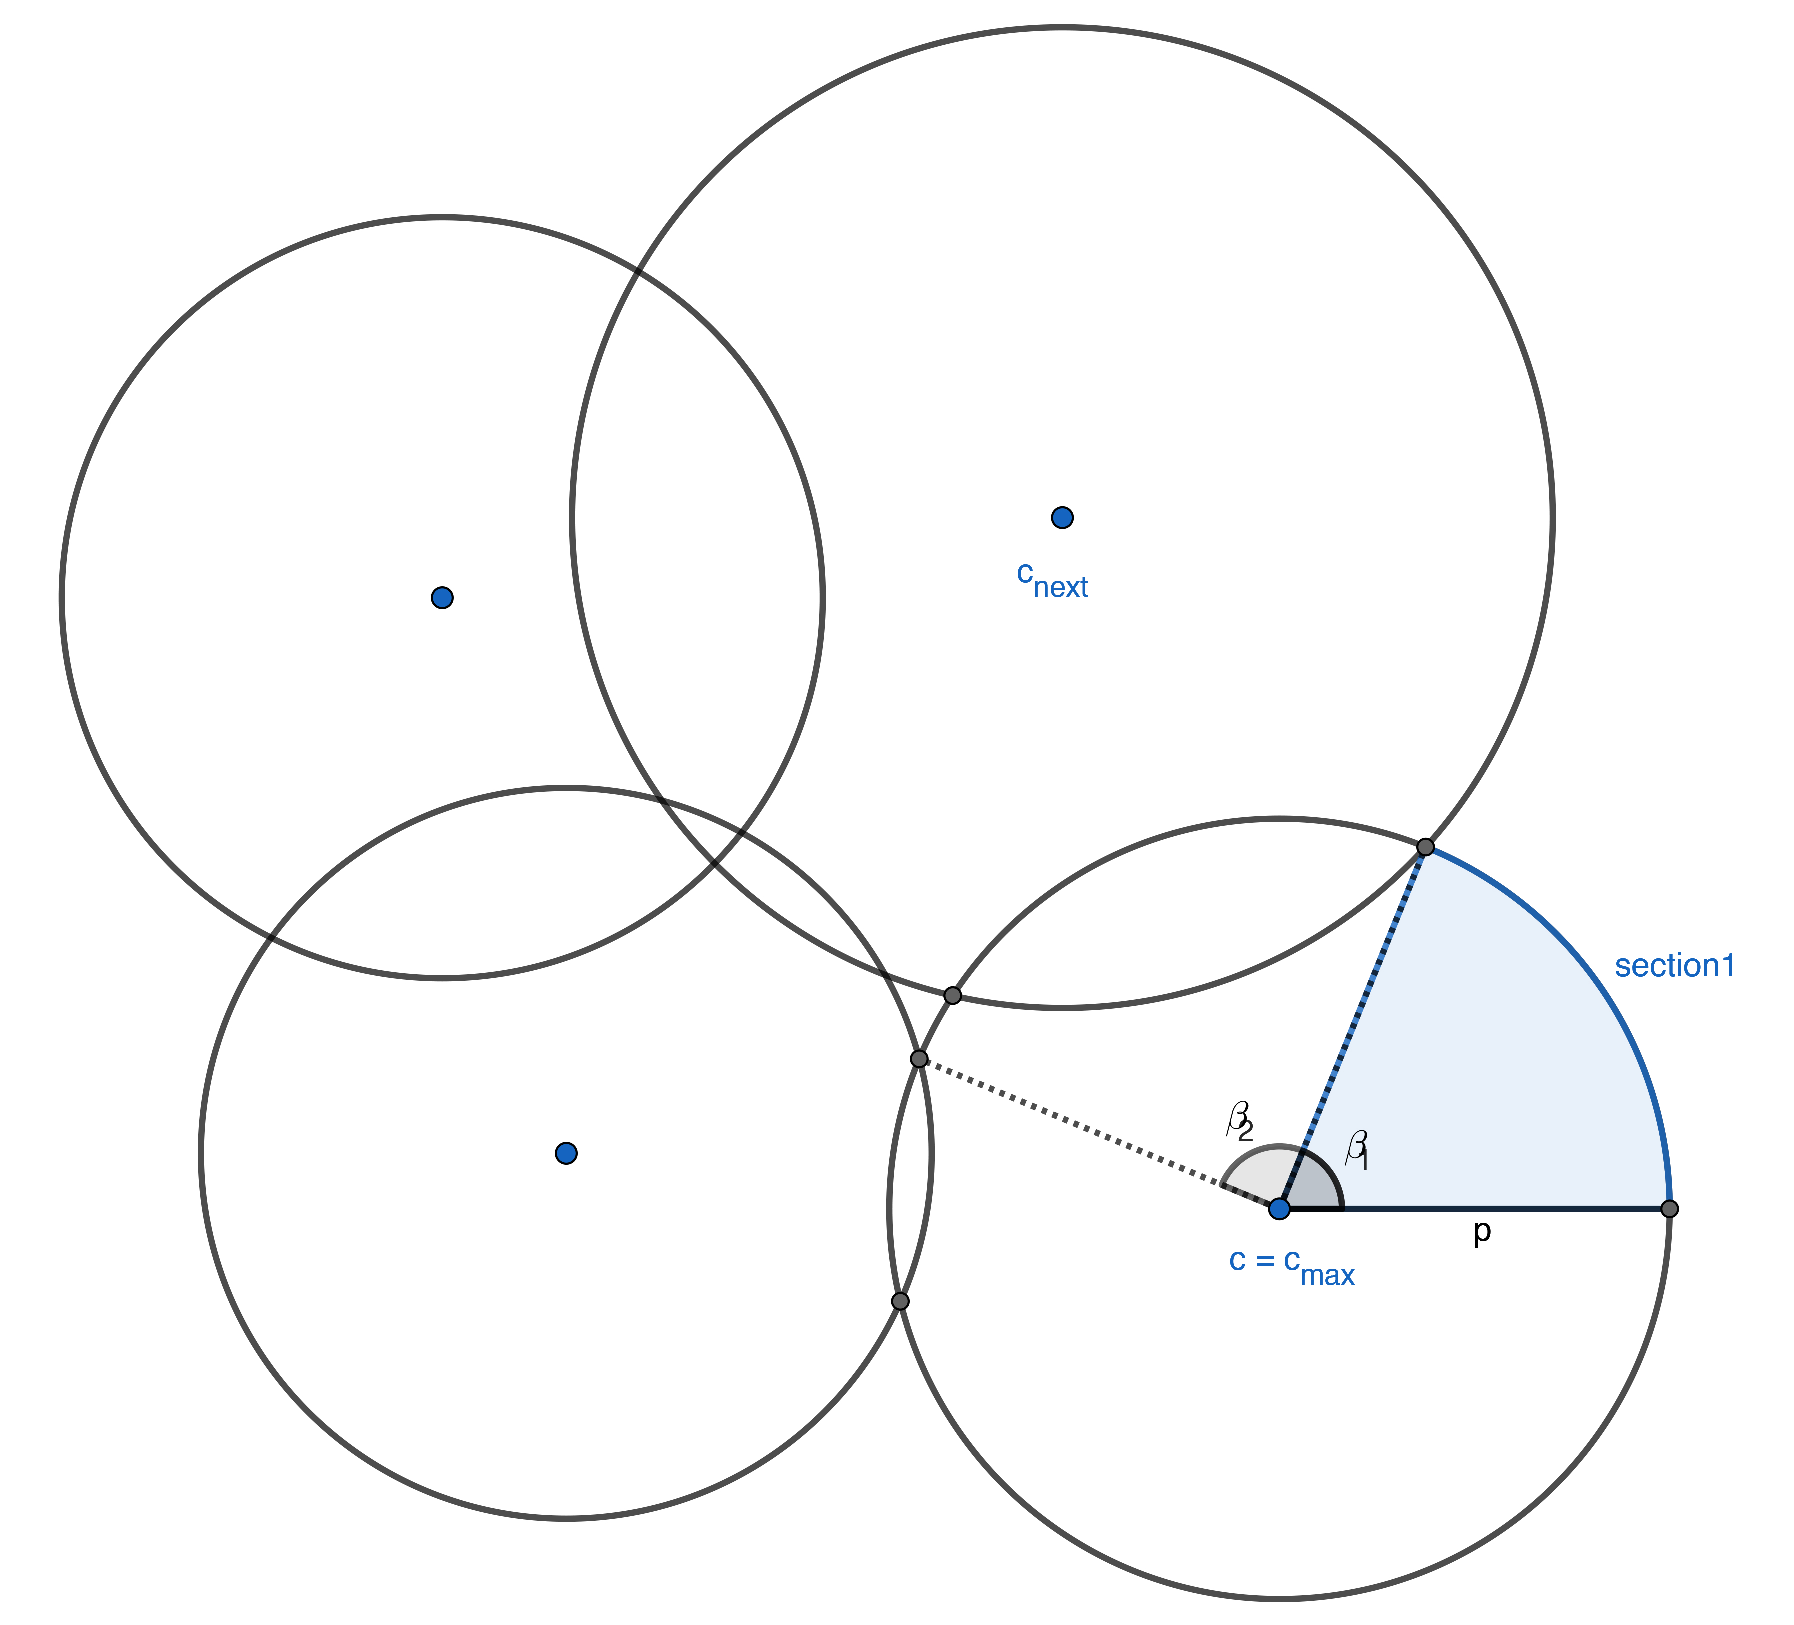
\includegraphics[width=1.0\textwidth]{figures/contour/c1copy.pdf}
    \caption{Finding first contour section}
  \endminipage\hfill
  \minipage{0.32\textwidth}
    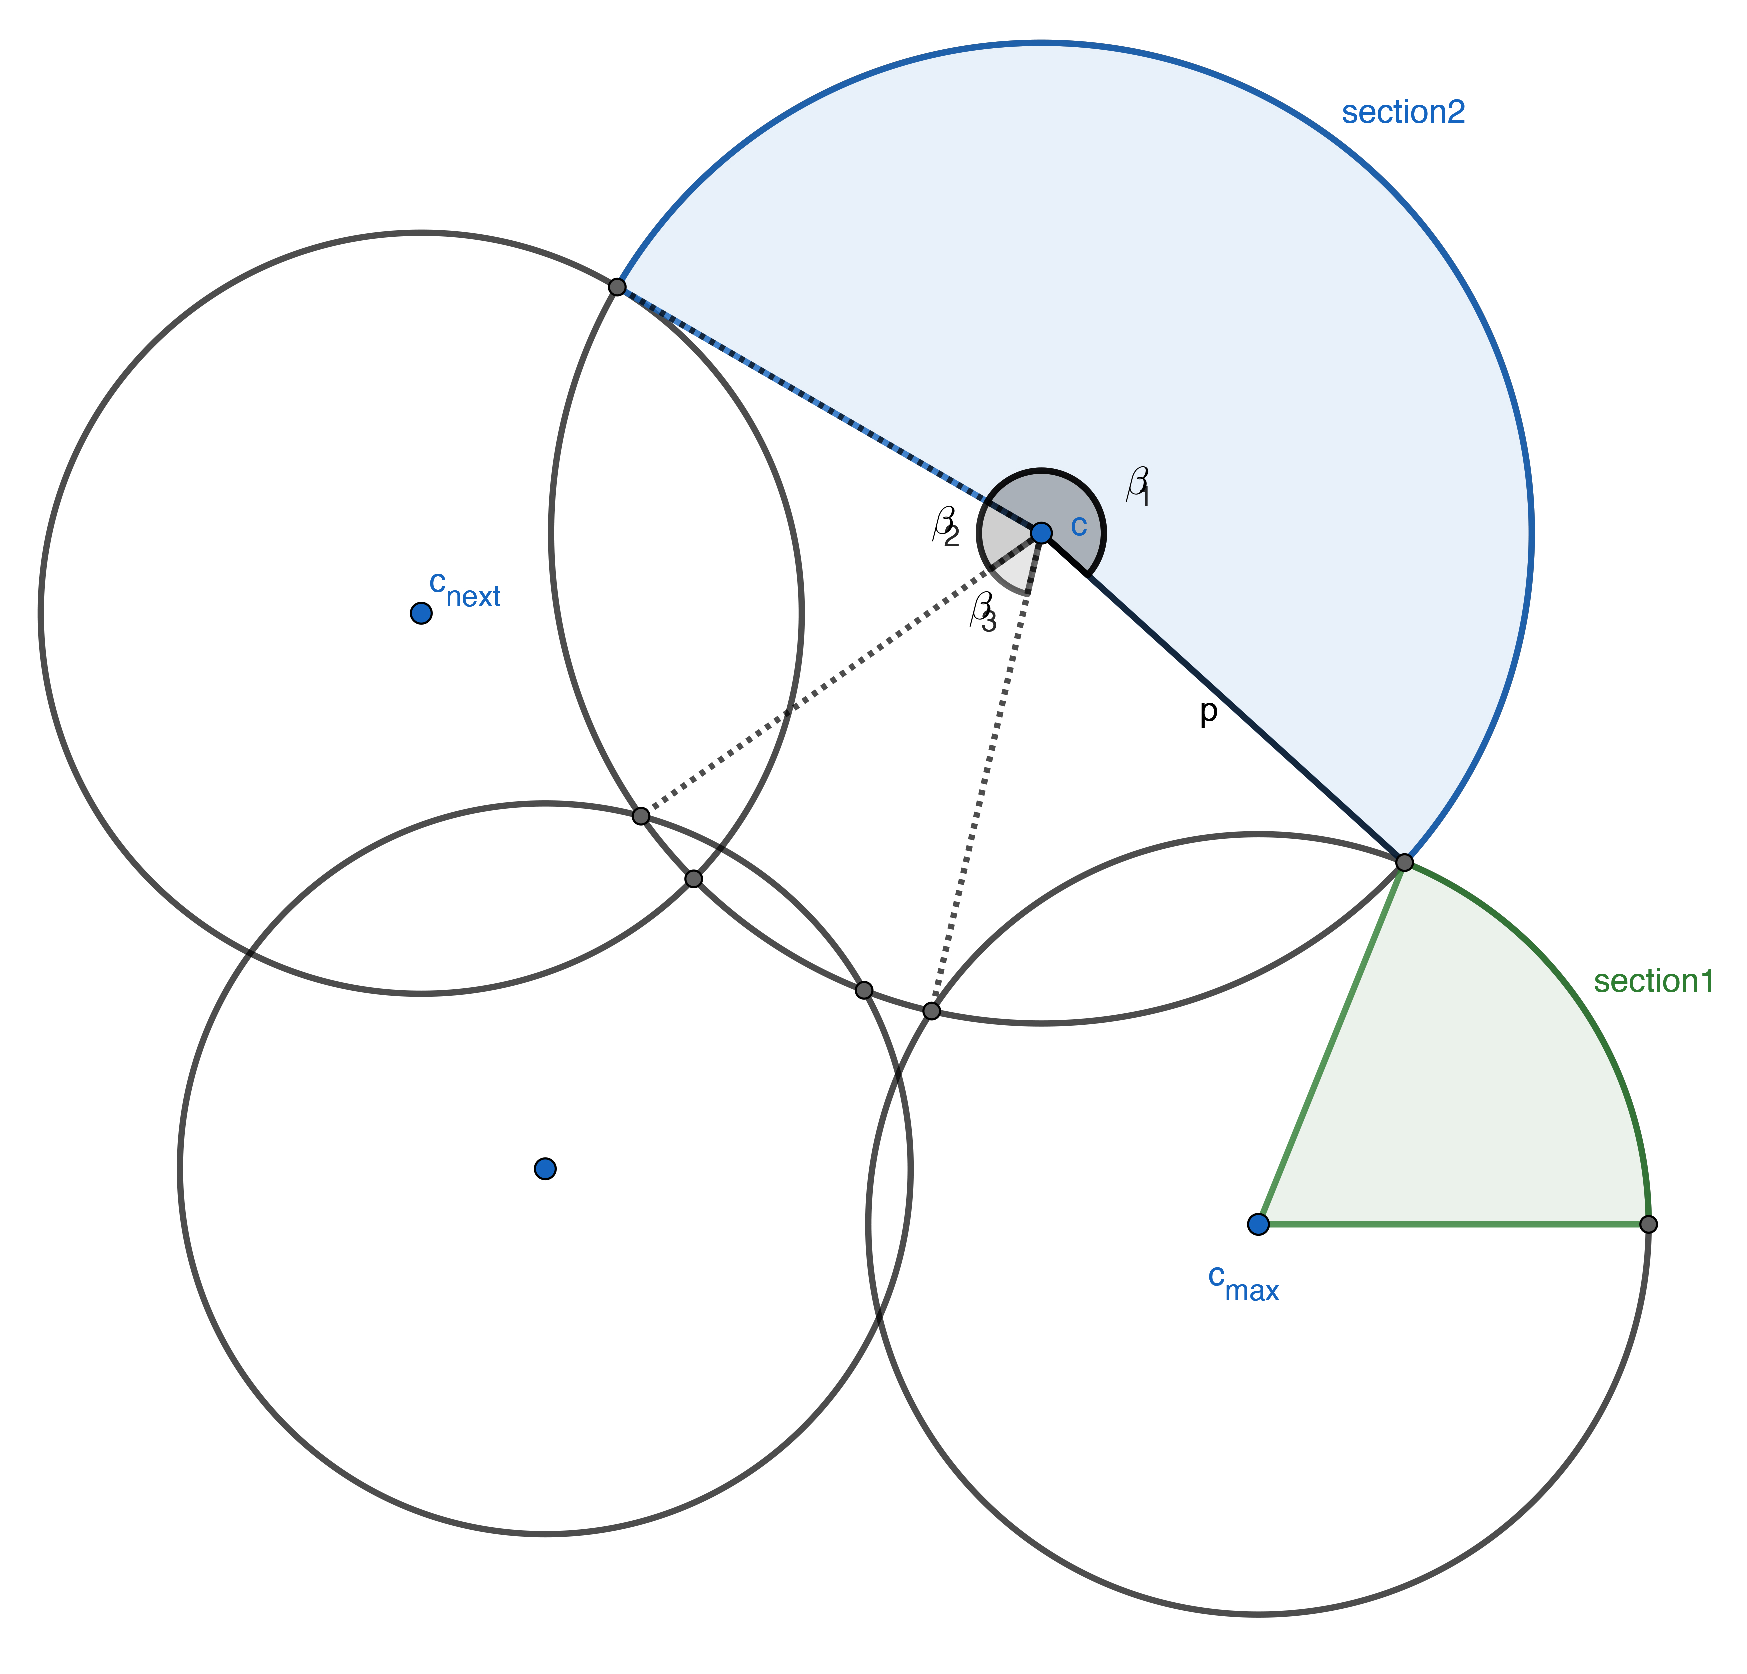
\includegraphics[width=1.0\textwidth]{figures/contour/c2copy.pdf}
    \caption{Finding middle contour section}
  \endminipage\hfill
  \minipage{0.32\textwidth}%
    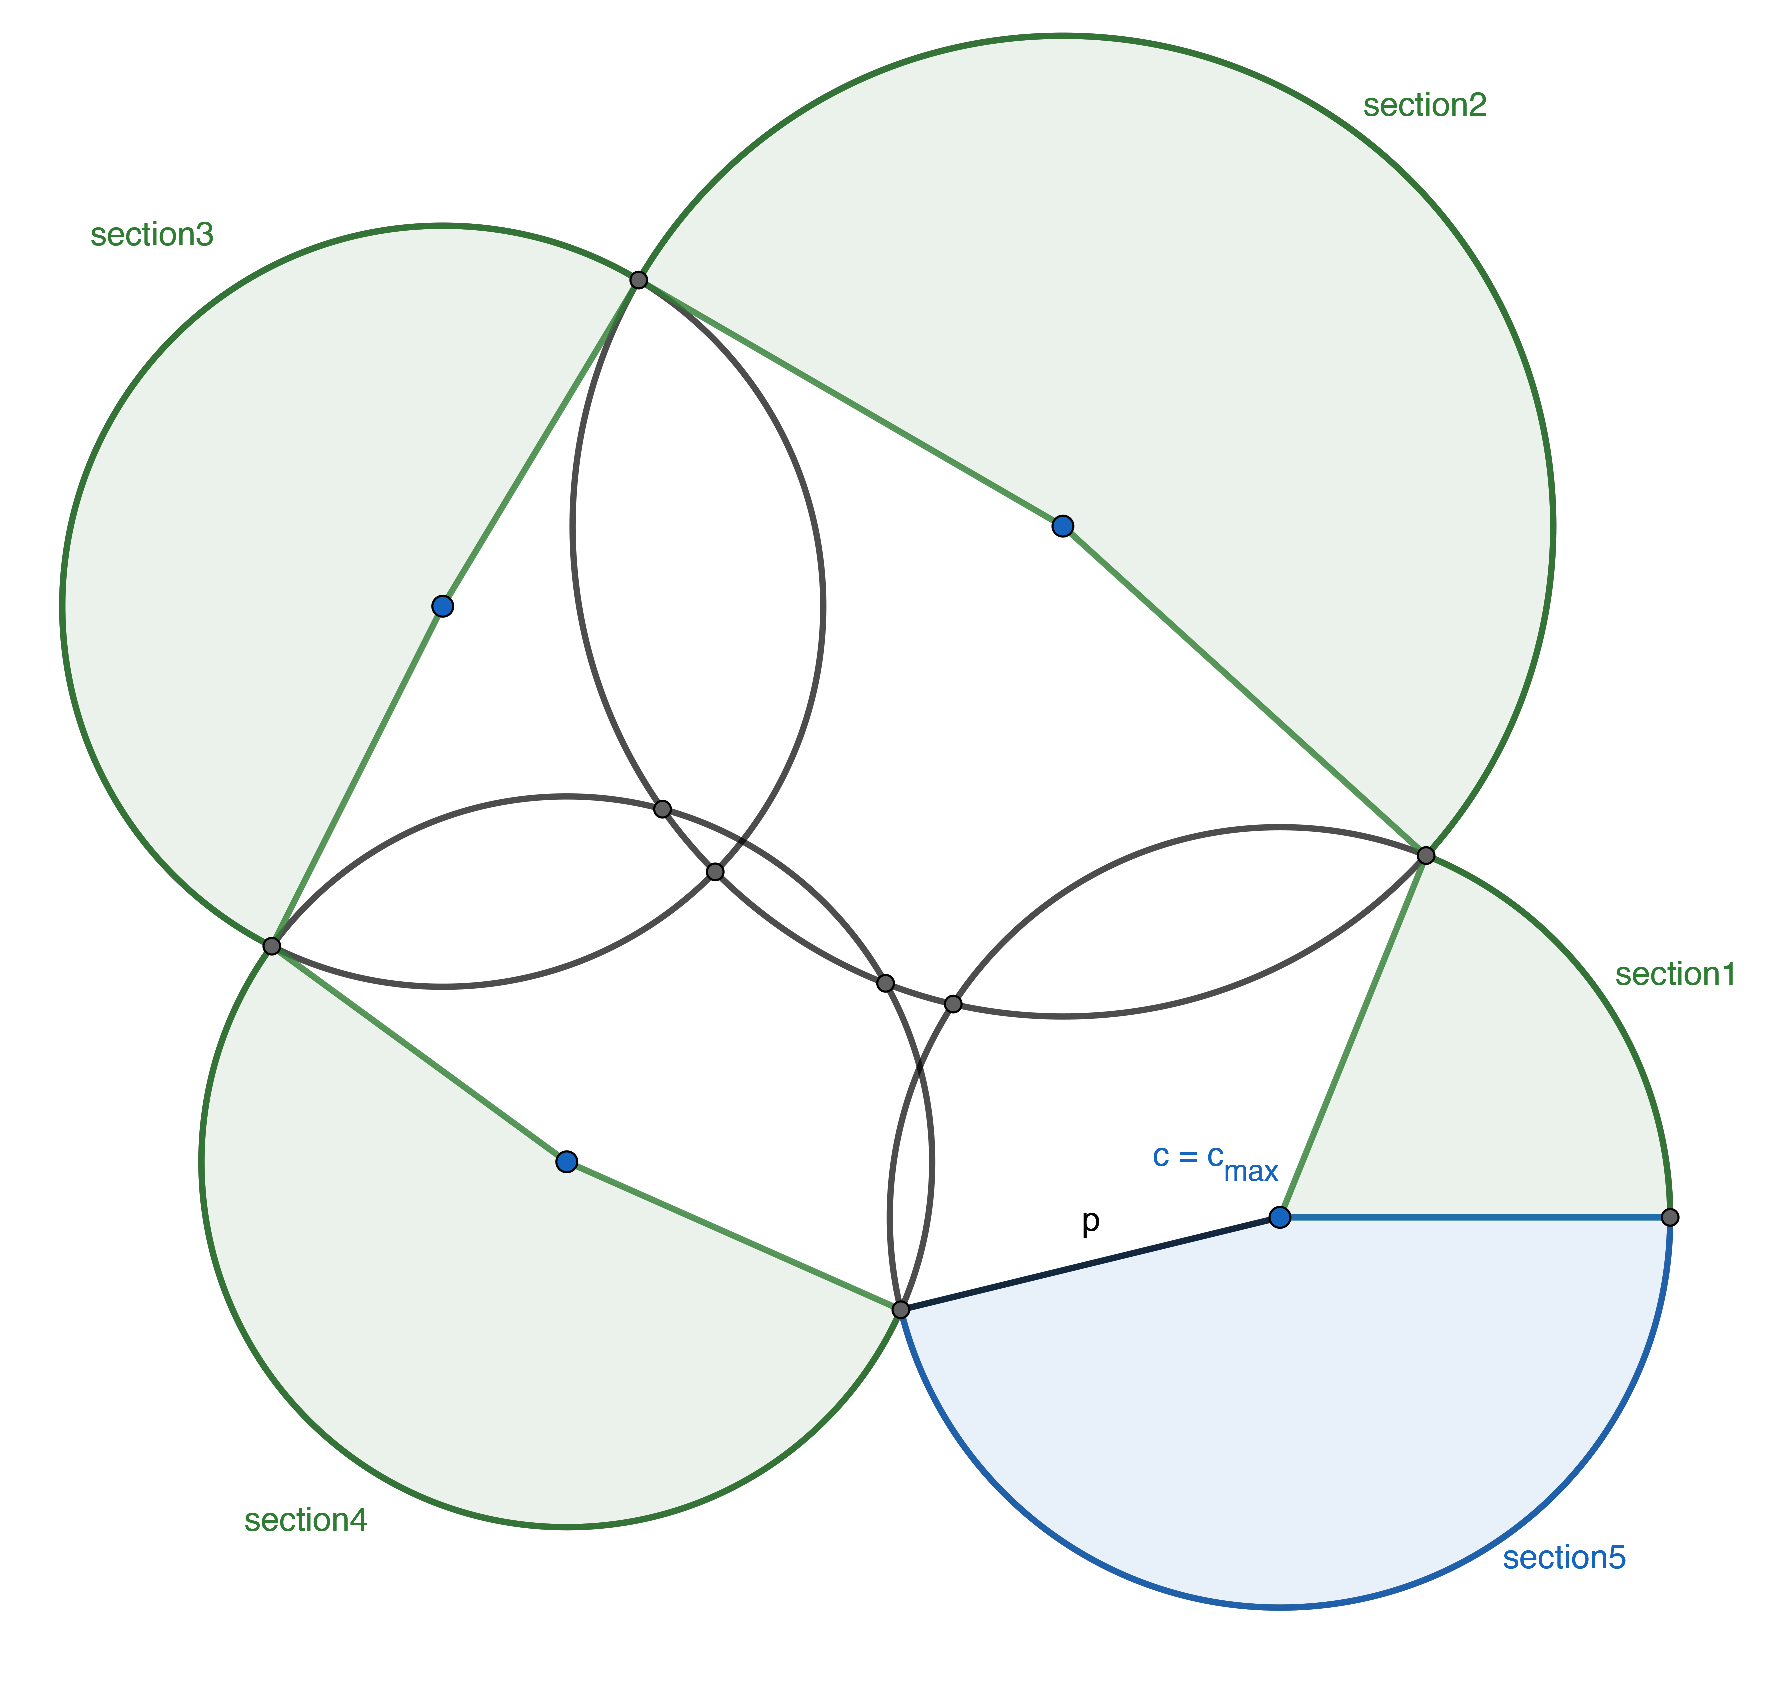
\includegraphics[width=1.0\textwidth]{figures/contour/c3copy.pdf}
    \caption{Finding the last contour section}
  \endminipage
  \caption[Visualization of CircleSetContour algorithm]{Visualization of \autoref{alg:CircleSetContour}}
  \label{fig:circlesetcontour}
\end{figure}


\subsection{Elliptic fourier descriptor}

Now that we have a contour for each slice, we'll use the elliptic fourier descriptor (EFD) to describe that contour.
EFDs allow for a high resolution encoding of a contour in a fixed amount of coefficients.
Additionally, EFD coefficients can easily be made rotationally invariant.

EFDs, as described in \cite{LIN1987535} work by selecting a random starting point $s$ on the contour.
Starting from $s$, we will follow the contour and denote the $x$ and $y$ coordinates as functions $x(l)$, $y(l)$ of the distance $l$ from the starting point.
Distance refers to the length it takes to get from $s$ to the point following the contour.

Since the starting and end point of $x(l), y(l)$ will be equal, making them periodic, we can define a parameter $t=\frac{2\pi l}{n}$. %TODO: Erklären!!!!
The functions can then be described by Fourier expansions as

%TODO: Replace t and put it in directly?
$$
\begin{pmatrix}
  x(l) \\
  y(l) \\
\end{pmatrix}
=
\begin{pmatrix}
  a_0 \\
  d_0 \\
\end{pmatrix}
+
\sum_{k=1}^\infty 
\begin{pmatrix}
  a_k & b_k\\
  c_k & d_k\\
\end{pmatrix}
\cdot
\begin{pmatrix}
  \cos(kt)\\
  \sin(kt)\\
\end{pmatrix}
$$

with

$$
a_0 = \frac{1}{2\pi} \int_{0}^{2 \pi}  x(t) \,dt 
$$
$$
d_0 = \frac{1}{2\pi} \int_{0}^{2 \pi}  y(t) \,dt 
$$

$$
a_k = \frac{1}{\pi} \int_{0}^{2 \pi}  x(t) \cos(kt) \,dt 
$$
$$
b_k = \frac{1}{\pi} \int_{0}^{2 \pi}  x(t) \sin(kt) \,dt 
$$
$$
c_k = \frac{1}{\pi} \int_{0}^{2 \pi}  y(t) \cos(kt) \,dt 
$$
$$
d_k = \frac{1}{\pi} \int_{0}^{2 \pi}  y(t) \sin(kt )\,dt 
$$

The $a_k, b_k, c_k, d_k$ form a basis for the functions $x(l), y(l)$.
By addition of the vector $ \begin{pmatrix} a_0 & b_0 \end{pmatrix}^T $ a center offset can be defined.
Since the contours encoded here should stay rotationally invariant, a two dimensional offset is not feasible.
Instead the offset length $\|  \begin{pmatrix} a_0 & b_0 \end{pmatrix}^T \| $ is added to the feature vector.

So far, the features $a_k, b_k, c_k, d_k$ are depended on the rotation of the contour.
The next step will be to make the features invariant under rotations.
%%%The starting point $s$ does not affect the coefficients as shown by \citeauthor{KUHL1982236}.

The contour can be viewed as a summation of ellipses of different size.
By aligning the first ellipse and rotating all other ellipses accordingly, the final output can be made invariant
of rotation \cite{MEBA}.

$$
\theta = \frac{1}{2}\arctan \left( \frac{2(a_1b_1 + c_1d_1)}{a_1^2 + c_1^2 - b_1^2 - d_1^2} \right)
$$
$$
\psi = \arctan \left( \frac{\cos(\theta) a_1 + \sin(\theta) b_1 }{\cos(\theta) c_1 + \sin(\theta) d_1} \right)
$$

The aligned coefficients $a_k^R, b_k^R, c_k^R, d_k^R$ can then be obtained using

$$
\begin{pmatrix}
  a_k^* & b_k^* \\
  c_k^* & d_k^* \\
\end{pmatrix}
=
\begin{pmatrix}
  \cos(\psi) & -\sin(\psi) \\
  \sin(\psi) & \cos(\psi) \\
\end{pmatrix}
\begin{pmatrix}
  a_k & b_k \\
  c_k & d_k \\
\end{pmatrix}
\begin{pmatrix}
  \cos(k\theta ) & -\sin(k\theta) \\
  \sin(k\theta) & \cos(k\theta) \\
\end{pmatrix}
$$.

The rotation around $\theta $ can be interpreted as normalizing the starting point $v$, 
the rotation around $\psi$ as normalizing the rotation of the contour itself \cite{KUHL1982236}.

The last step is to choose an order up to which the contour is approximated.
At the moment the infinite sum ensures a perfect approximation original contour. 
By limiting the coefficients to an order $k_{max}$ the number of coefficients describing our contour can be limited.
Generally, the higher the order, the better small changes in the contour can be approximated Figure~\ref{fig:slice-layered}.

After normalizing, the values $b_1^* = c_1^* = 1$ will always be equal to 0, since we rotated the first ellipse to be aligned.
We can therefore remove $b_1^*, c_1^*$ from the feature vector.

After calculating the coefficients for every slice, the different slices will be concatenated into a 2D array.
One dimension of the array will correspond to the spacial $z$ direction, so it will be equivalent to the number of layers chosen.
The other dimension will hold the fourier coefficients for each layer.

To keep information about the offset from the center, the length $l = \| \begin{pmatrix} a_0 & b_0 \end{pmatrix} \| $ will be added for each slice.
Since each fourier coefficient consists of 4 values and $b_1^*, c_1^*$ are removed while the center offset $l$ is added, the size of this dimension will be $k_{max} * 4 - 1$.

These features will be used for prediction of a molecules activation barrier in the next step.

\begin{figure}[h]
  \minipage{0.4\textwidth}
    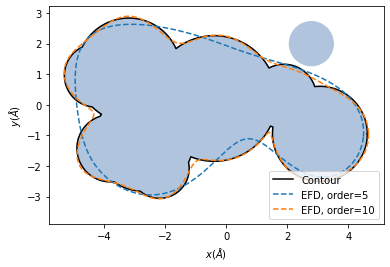
\includegraphics[width=1.0\textwidth]{figures/fourier/contour.png}
  \endminipage\hfill
  \minipage{0.6\textwidth}
    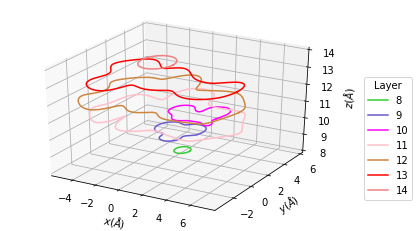
\includegraphics[width=1.0\textwidth]{figures/fourier/fourier-slices.png}
  \endminipage
  \caption[Slices produced by LEFD encoder]{
  On the left a slice is described by fourier descriptors. Higher order descriptors are able to approximate the contour better than lower order descriptors. 
  The isolate is ignored by the contour descriptor. The rotation is kept as part of the fourier description for illustration purposes.
  On the right the different slices making up on element are placed on top of each other. Slices without any volume are not rendered. 
  Wile the rotation is removed to keep it rotationally invariant, the offset from the center is encoded.
  }
  \label{fig:slice-layered}
\end{figure}

\section{Feature generation using smooth normalized atomic positions}
\label{ch:SNAP}
In a second approach, the molecule was encoded by smoothing the atomic positions, 
and then combining a set of functions describing the 3D space around the metal center.

This method is similar to the Smooth Overlap of Atomic Positions (SOAP) descriptor, that produces a 
fully rotational invariant description for the space surrounding one or more atomic centers \cite{Bart_k_2013}.
Specifically the gaussian smoothing of atomic positions and combination of radial basis functions with
spherical harmonics to describe a 3D space is taken from SOAP.
While SOAP describes the overlap of densities for different species, the goal here is to describe the density space directly.
The disadvantage of SOAP is that due to the rotational invariance, the 3D environment cannot be reconstructed from the generated features.
Due to the similarities between SOAP and SNAP, parts of the implementation and the following description of SNAP are based 
on the open-source library Dscribe that provides an implementation of SOAP \cite{dscribe}.

The Smooth Normalized Atomic Positions (SNAP) descriptor proposed here allows for a reconstruction of the 3D space from the coefficients, 
while partly keeping the rotational invariance.
Rotational invariance however is not given by the feature generation itself, but rather by using the catalysts special struture.
The SNAP descriptor therefor is less universal than SOAP. 
In applications were no translation back to 3D space is required,
in most instances SOAP should be chosen over SNAP for it's fully rotationally invariant output.

\subsection{SNAP requirements}

The general idea of SNAP is to describe the atoms surrounding a cental atom using a fixed set of coefficients.
Rotational invariance therefore cannot be guaranteed, unless the encoded molecule itself can be rotated in a way to explicitly set it's rotation.

For catalyst molecules, this natural axis can be defined by setting the reaction pocket to the top, and the central iridium atom as a center.

For other molecule classes, defining a natural axis might not be as trivial.

When no clear axis of alignment can be found, the SNAP output may be augmented by rotating the input along all axis of freedom.
If there are multiple axis of freedom SOAP may be preferable since in naturally offers a fully rotationally invariant description.

Additionally, SNAP only encodes a local region within $r_{cut}$.
Density outside this cutoff radius is not considered.

If a global description of the entire element is needed, SNAP might not be the best option, especially when 
the size of the elements in the dataset varies a lot.

\subsection{SNAP}

Using the centered and aligned molecules, a density space surrounding the central iridium atom is defined.

By generating 3D gaussian distributions for every atom in the element, a density at any point within $r_{cut}$ can be calculated.
For each species $Z$ in the dataset, the density at any point $p = (x,y,z)$ is described as

$$\rho^Z(p) = \sum_i^{|Z|} w_{Z_i} e^{- \frac{1}{2\sigma^2} \vert p - R_i \vert^2 }$$  %TODO WAS IST SIGMA?

The summation $i$ runs over all the atoms of that species.
$R_i$ is the center of that atom.
$w_{Z_i}$ is a weight factor for each species. 
Since all species will be described independently of each other, for now all $w_{Z_i}=1$.
In further enhancements of the SNAP encoder, describing other molecular properties by adapting $w_{i}$ or the decay parameter $\sigma$ is possible.
Even describing 3D features not associated with a single species but rather describing the interaction or overlap of species 
or molecules are thinkable.

Since the basis set used to describe the space is using spherical coordinates, from now on
cartesian coordinated will be replaced by spherical coordinates.

$$
r = \sqrt{x^2 + y^2 + z^2}
,
\theta = \arccos(\frac{z}{r})
,
\varphi = \arctan(y / x)
$$ %TODO: Überprüfen

The density space can then be expanded using a combination of basis functions.
To expand the radial degrees of freedom, spherical harmonics are used.
Spherical harmonics are a complete set of orthonormal basis functions on spherical coordinates.
The spherical harmonics used here are the Laplacian Spherical Harmonics.
$$
Y_{lm}(\theta, \varphi) = (-1)^m \sqrt{\frac{2l + 1}{4 \pi} \frac{(l - m)!}{(l + m)!}} P_{lm}\left(\cos(\theta) \right) e^{im\theta}
$$

Here, $P_{lm}$ are the associated Legendre polynomials:

$$
P_{lm}(x) = (-1)^m (1-x^2)^{m/2} \frac{\partial^{l+m}}{\partial x^{l+m}}(x^2 - 1)^l
$$ %TODO: Looks at derivative


\begin{figure} [h]
  \centering
  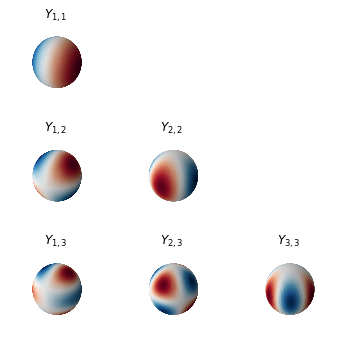
\includegraphics[width=0.5\textwidth]{figures/snap/sph-harm.png} % for .pdf files etc use \includegraphics{test.pdf}
  \caption[Spherical harmonics]{A selection of low order spherical harmonics plotted on a sphere. } %TODO: Add scale!!!
  \label{fig:sphharm}
\end{figure}

Using the spherical harmonics, a sphere surrounding the central atom can be encoded.
To encode density information along the radial direction, spherical harmonics are combined with radial basis functions.
A variety of radial functions can be used for this application.
In \cite{KUHL1982236} the use of a polynomial radial basis is suggested.
However here a set of primitive gaussian type orbitals are used.
This set allows for analytical integration which allows for a significant speedup over numerical integration since it can be precomputed \cite{dscribe}.
These gaussian type orbitals are defined as

$$g_{nl}(r) = \sum_{n'}{n_{max}} \beta_{nn'l} \phi_{n'lr}(r) $$

with 

$$\phi_{nl}(r) = r^l e^{-\alpha_{nl}r^2} $$ %TODO: phi of n oder phi of nl?? / alpha_n oder alpha_nl


\begin{figure} [h]
  \centering
  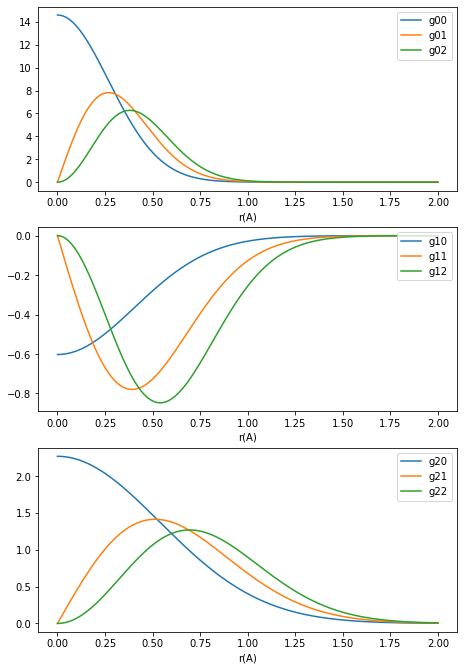
\includegraphics[width=0.5\textwidth]{figures/snap/gaus_orb.png} % for .pdf files etc use \includegraphics{test.pdf}
  \caption[Radial basis functions]{Spherical gaussian orbital functions for a cutoff radius $r_{cut}=2$, $2$, $n_{max}=2$ and $l_{max}=2$. }
  \label{fig:gaussians}
\end{figure}

$\alpha$ and $\beta$ are constants that only need to be computed once for every pair of $l,m, r_{cut}$.
The $\alpha$ parameters control the decay of the radial basis functions at $r_{cut}$.

$\beta_{nn'l}$ parameters orthogonalize the radial basis functions.
For each $l$ the weights $\beta_{nn'l}$ can be computed using the Löwdin orthogonalization:

$$\beta = S(l)^{-1/2} $$

with the entries of the matrix $S$ being defined as

$$S(l)_{nn'} = \langle \phi_{nl} | \phi_{n'l} \rangle  $$

The implementation of $\alpha$ and $\beta$ prefactors is taken from \cite{dscribe} where they are precomputed up to $l \leq 9$.
Higher order factors could be added if needed.


Combining spherical harmonics with radial basis functions the density space surrounding the central atom can be described.
In theory, choosing infinitely high $n, l$ could approximate the space with infinitely high precision.
To get a fixed amount of coefficients, $n_{max}$ and $l_{max}$ need to be chosen that determine the
accuracy of the encoding.
Generally, the higher $n_{max}, l_{max}$ the more accurate the space can be approximated.
%TODO Add figure of the space being described with different n, l , cutoff

For radial basis functions a cutoff radius $r_{cut}$ needs to be defined.
Densities outside this cutoff radius will not be encoded in the features of the space.

The density for every species $Z$ in within the cutoff sphere can be expanded as:

$$ \rho^Z(r) = \sum_{nlm} c^Z_{nlm} g_{nl}(r) Y_{lm}(\theta, \varphi) $$

The coefficients $c_{nlm}^Z$ are features generated by the SNAP descriptor.

$$ c_{nlm}^Z = \iiint_{R^3} g_{nl}(r) Y_{lm}(\theta, \varphi) \rho^Z(r, \theta, \phi)  \,dr\theta\phi   $$
% TODO: Integrate to infinity or r_cut?

The 3 dimensional integral goes over all spherical coordinates within the cutoff sphere.
The coefficients $c^Z_{nlm}$ now describe the 3D space within a fixed size sphere.
\\
The key difference between SNAP and other chemical descriptors is the bi-directional mapping between feature space and 
density space.
From the coefficients, the density space encoded can be easily reconstructed.
This allows for a partial reconstruction of the molecule from the features encoded by SNAP.

However, due to the low number of radial basis functions and spherical harmonics usually used to describe an element, 
the encoding of the density is far from perfect.
While with an infinite amount of coefficients a perfect description of the space is thinkable,
in reality the computational limits only allow for a rather low resolution of the density space [Figure~\ref{fig:snap-density}]. 
\begin{figure} [h]
  \centering
  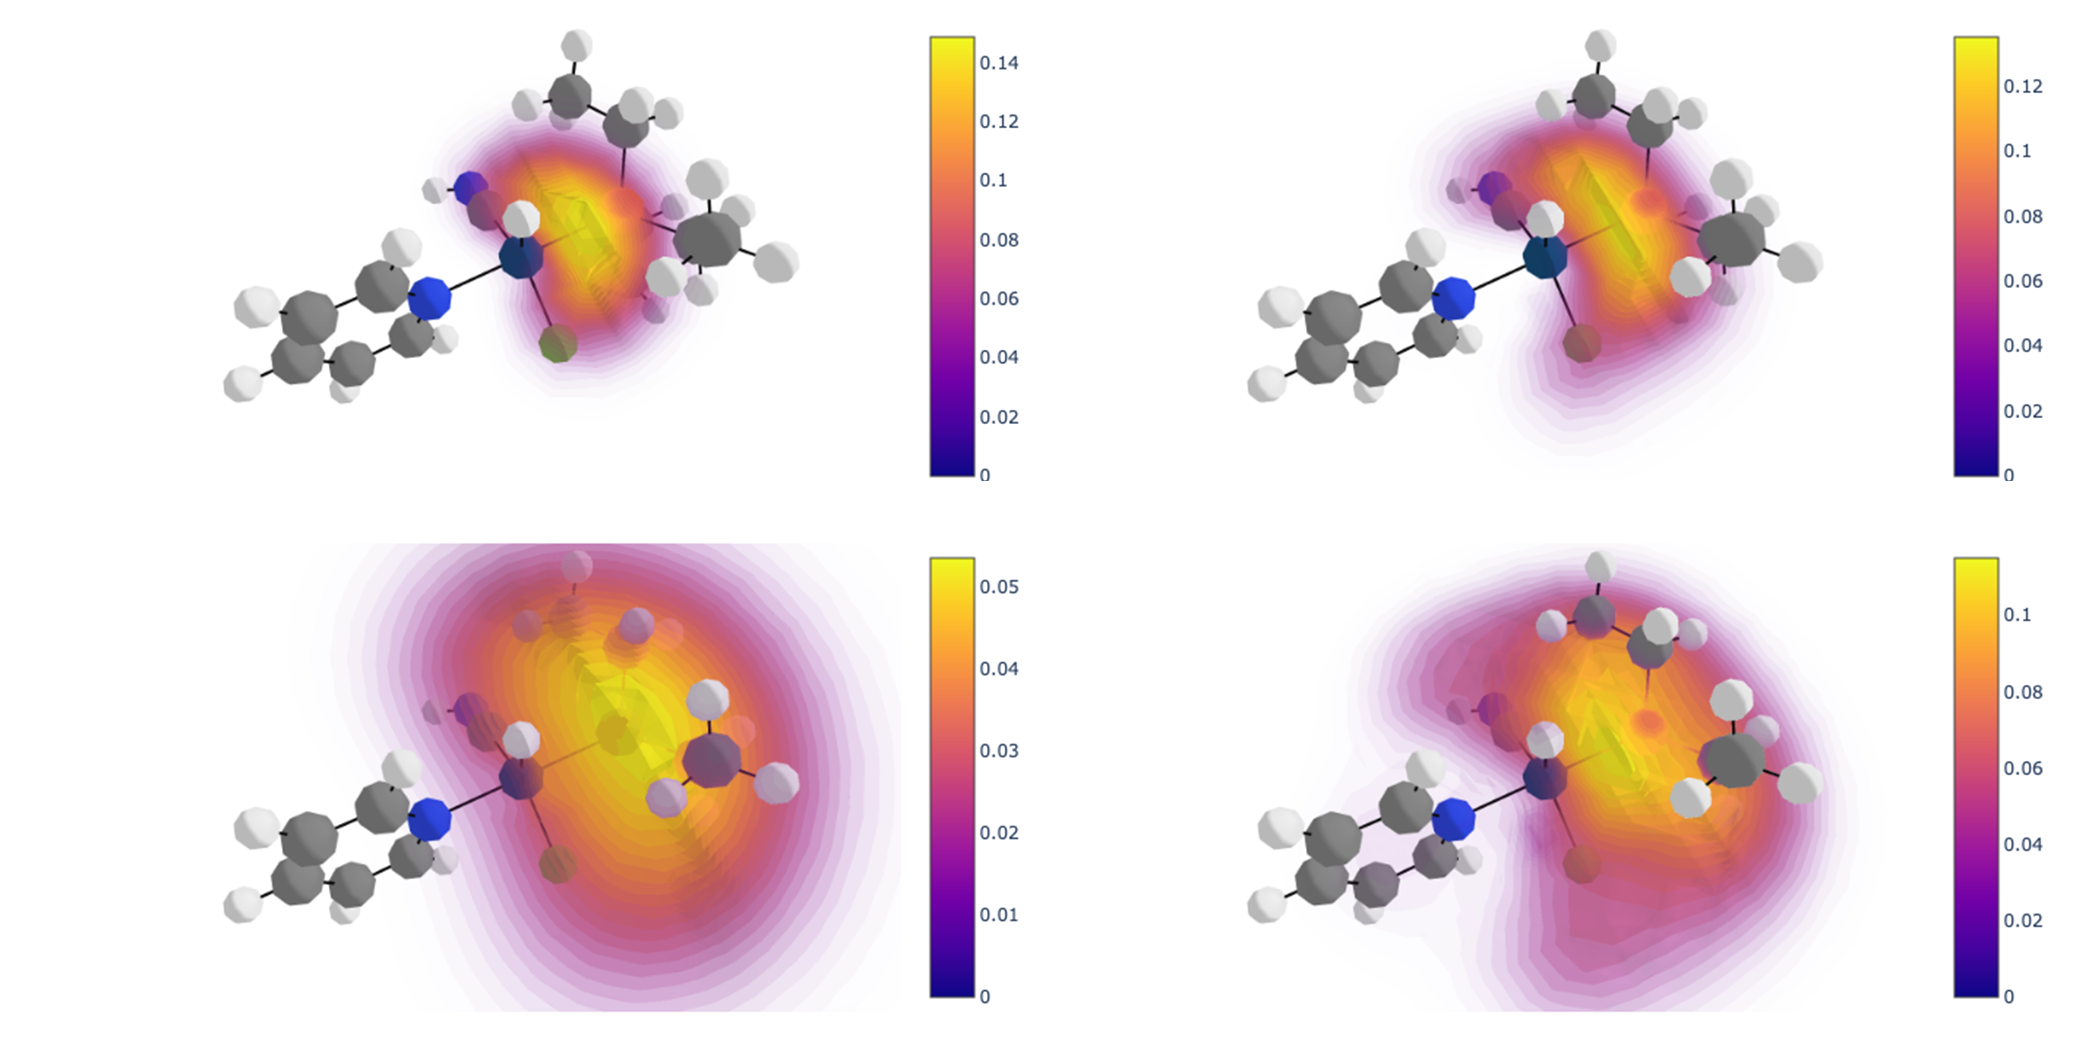
\includegraphics[width=1\textwidth]{figures/snap/density/dense.png} % for .pdf files etc use \includegraphics{test.pdf}
  \caption[SNAP density visualization]{Visualization of the density reconstructed from $c_{nlm}^Z$ coefficients for different resolutions.
  Top: $r_{cut} = 10$, bottom: $r_{cut} = 25$, left: $n_{max} = l_{max} = 2$, right: $n_{max} = l_{max} = 8$.
  The density shown is visualizing the density for phosphorus only.
  The phosphorus atom is the orange atom surrounded by the density cloud.
  }
  \label{fig:snap-density}
\end{figure}

This means that in many cases, the center of the encoded density and the center of the atom do not match.
Especially when the element contains many atoms of one species, the descriptor struggles to fully encode the space.

Despite these issues, predicting the activation barrier from SNAP features is still possible with high accuracy.
The interpretability of these results however is limited to a low resolution.
When using network explainers in combination with SNAP coefficients, this limited accuracy needs to be kept in mind.

%% LaTeX2e class for student theses
%% sections/evaluation.tex
%% 
%% Karlsruhe Institute of Technology
%% Institute for Program Structures and Data Organization
%% Chair for Software Design and Quality (SDQ)
%%
%% Dr.-Ing. Erik Burger
%% burger@kit.edu
%%
%% Version 1.3.5, 2020-06-26

\chapter{Regression}
\label{ch:Regression}

After extracting features from the elements, the next step is do learn from the data.
The goal of this Bachelor's thesis is to predict the activation barrier of a catalyst molecule.
The techniques used however are not limited to the activation barrier, 
as it can be expected that other properties of the molecule could be predicted with similar techniques.

For regression, artificial neural networks(ANNs) will be used.
Neural networks have seen a huge surge in popularity in recent years for their ability to well
adapt to high dimensional input data.
The concept is derived from biological neural networks such as the ones found in the human brain.

ANNs are a composed of a set of interconnected neurons.
Each neuron has a set of inputs $x_1 .. x_n$, a bias $b$, and an activation function $f(x)$.
The output will be the result of the activation function applied to the sum of all inputs plus the bias.

Neurons are grouped together in layers, where the output of each layer is connected to the input of the next one.
For a single prediction, the example is applied to the input layer, the network is then flooded until the output layer is reached.
In the case of regression used here, the value of the output layer is the prediction of the neural network.

% Listing 2: Tex for neural network pipeline
\begin{tikzpicture}[
    % define styles    
    init/.style={ 
         draw, 
         circle, 
         inner sep=2pt,
         font=\Huge,
         join = by -latex
    },
    squa/.style={ 
        font=\Large,
        join = by -latex
    }
]
% Top chain x1 to w1
\begin{scope}[start chain=1]
    \node[on chain=1] at (0,1.5cm)  (x1) {$x_1$};
    \node[on chain=1,join=by o-latex] (w1) {$w_1$};
\end{scope}
% Middle chain x2 to output
\begin{scope}[start chain=2]
    \node[on chain=2] (x2) {$x_2$};
    \node[on chain=2,join=by o-latex] {$w_2$};
    \node[on chain=2,init] (sigma) {$\displaystyle\Sigma$};
    \node[on chain=2,squa,label=above:{\parbox{2cm}{\centering Activation\\ function}}]   {$f_{act}$};
    \node[on chain=2,squa,label=above:Output,join=by -latex] {$y_{out}$};
\end{scope}
% Bottom chain x3 to w3
\begin{scope}[start chain=3]
    \node[on chain=3] at (0,-1.5cm) 
    (x3) {$x_3$};
    \node[on chain=3,label=below:Weights,join=by o-latex]
    (w3) {$w_3$};
\end{scope}
% Bias
\node[label=above:\parbox{2cm}{\centering Bias \\ $b$}] at (sigma|-w1) (b) {};
% Arrows joining w1, w3 and b to sigma
\draw[-latex] (w1) -- (sigma);
\draw[-latex] (w3) -- (sigma);
\draw[o-latex] (b) -- (sigma);
% left hand side brace
\draw[decorate,decoration={brace,mirror}] (x1.north west) -- node[left=10pt] {Inputs} (x3.south west);

\end{tikzpicture}


Finding a good performing network architecture is challenging. \\
Since generally no rule is known on what neural network architecture will work best on the given data, the space of possible networks needs to be explored.
A variety of choices for the network architecture can be made, such as the amount of layers, size of the layers, type of activation functions, regularization, normalization, and many more.

When choosing the network architecture, generally a bigger network will be able to adapt to more complex data.
However if the network will become to big, it might encounter issues with overfitting.
Overfitting is a problem encountered when the network adapts to the training data too well.
This will decrease it's ability to generalize the data and make good predictions on previously unseen samples Figure~\ref{fig:overfitting}.

Measure to counteract overfitting include regularization and dropout layers.
Regularization introduces a penalty term that punishes the network for extreme values.
This causes the network to adapt less well to the training data, but in return can help with the network
performance on previously unseen data.

Dropout layers randomly disable neurons in a layer.
This forces the network to be less reliant on certain neurons, and instead learn the data in the entire network.
\\

To find a suitable network architecture, a hyperparameter optimization needs to be performed.
Hyperparameter optimization aims to find a good performing network architecture by testing the performance
of different networks on the data.
%TODO: Mehr?

\begin{figure} [h]
    \centering
    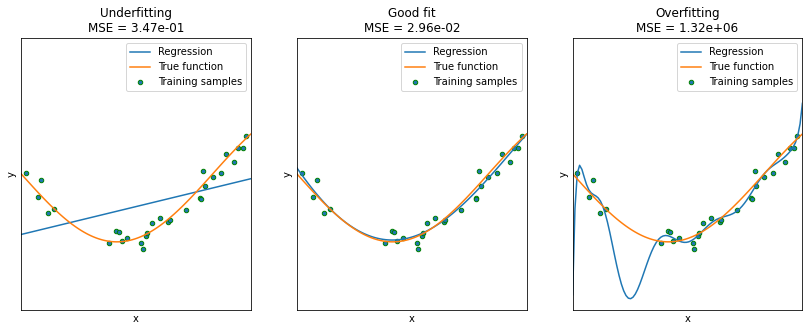
\includegraphics[width=0.9\textwidth]{figures/regression/overfitting.png} 
    \caption[Overfitting]{Regression on a function with training examples. 
            The underfitting model is not complex enough to fit to the data well. 
            The overfitting model is too complex for the data.
            While the training error is lower for the overfitting model, 
            the overall performance of the overfitting model on previously unseen data 
            is worse than for the model with a good fit.
        }
    \label{fig:overfitting}
\end{figure}
  
To prevent overfitting while still getting good regression results, multiple network architectures need to be considered.
The networks proposed here were found by a manual exploration of the network architecture first.
In a second step, hyperparameter analysis was run to find a good network architecture.

\paragraph{Technicalities}

All networks were generated in Keras, an open-source deep learning library.
Keras offers a high level Python API to create, train and analyse neural networks.

To allow for better training and predictions, all features and labels were standardized before being passed to the neural network.
Standardizing is a process where each feature $f$ is scaled to independently so the mean over all samples in the dataset is 0, 
and the every feature has unit variance.
This can easily be achieved by independently subtracting the mean $\overline{f}$ over all samples, and dividing by the standard deviation $\sigma_f$.

$$
f_{norm} = \frac{f- \overline{f}}{\sigma_f}
$$

The same scaling is applied to the labels.
This means the networks do not directly predict the activation barrier, but the networks prediction needs to be scaled back first.

Hyperparameter optimization was performed using keras-tuner, a hyperparameter tuner for Keras.
Keras-tuner offerers a variety of different algorithms.
In the hyperparameter optimizations performed here, Keras Hyperband was used.
Keras Hyperband is an  implementation of the Hyperband algorithm propsed in \cite{li2017hyperband}.
It focuses on an optimized search speed compared to other Hyperparameter optimization methods, such as
Bayesian Optimization, by adaptive resource allocation and early stopping.

Hyperparameter optimization took multiple hours for LEFD features, 
and multiple days for SNAP features.
Training and hyperparameter optimization was performed on the universtiy cluster %TODO: Notwendig?
using a Nvidia Tesla V100-SXM2-32GBa GPU.

During training and hyperparameter optimization, a fraction of the data was reserved as test set.
This test set was not used for training or validation, but only to evaluate the final performance of the networks.
All data about network performance in this chapter is measured on the test set, unless specified otherwise.

During training of a network it is common practice to reserve a validation split that is not used to train the network.
Instead, the networks performance is measured on the validation data, and tuned to achieve similar accuracies on
training and validation data.
This helps to avoid overfitting in the network, since the network can no longer just memorize the training
data, but instead has to achieve good performance on data not seen during training as well.

This means there is a total of 3 datasets, one being used for training, the other being used to validate the networks
performance during and after training, and the last being used after hyperparameter optimization to evaluate the final network
performance.

\section{Regression on fourier descriptor features}
\label{sec:Evaluation:fourier}

In the first approach, the features generated by the fourier descriptor were used.
Notable hyperparameters to the feature extractor here are the number of layers $l$ and the order $o$ of the fourier descriptor.

The start and end height of the layers are chosen so that all the molecules in the dataset fully fit within $z_{min}$ and $z_{max}$.

The output shape of the descriptor will be an array of size $l \times (o * 4 - 1)$.
Generally, the bigger the number of fourier coefficients, the better the contour can be approximated.
However, an order that is chosen too high may increase the risk of overfitting.
This problem is commonly referred to as "the curse of dimensionality". %TODO Rausschmeißen?

The highest accuracy of prediction is not the only metric to be considered when choosing these hyperparameters.
Since the ultimate goal is not to get the most accurate prediction possible, but instead discover which parts of 3D space 
are responsible for prediction, an order that offerers reasonable high accuracy of prediction and 
allows for an interpretation of the feature space needs to be found.

After various tests with multiple orders, an order of $k_{max} = 10$ seemed to be a good compromise between accuracy of description and accuracy of prediction.
The following results will be focused on an order of $10$.

The same problem is faced when defining the number of slices.
Here the problem becomes more tricky, since the number of slices seems to play a huge part in the architecture of the ANN used.
This means hyperparameter analysis needs to be performed individually for every choice of the number of layers.

Since every slice is composed of same kind of fourier coefficients, the first idea was to use convolution layers to decrease the dimensionality of the input.
Filters might be able to recognize structures in each of the slices, and applied them across the different slices.

Convolution layers heavily depend on the assumption that the relative location of the features matters.
Filter sizes were therefore chosen to correspond to the dimensions over which similarities in the structures of the features are expected.
In the case of fourier coefficients, the filter therefore were only stretched along the dimension of the different $z$ layers, and not along the dimension of the fourier descriptors.

Multiple tests were performed with various filter sizes and convolution layers.
The regression accuracy was falling short of expectations, and the general shape of the convolution part of the network did not seem to change the prediction accuracy significantly.

\begin{figure} [h]
    \centering
    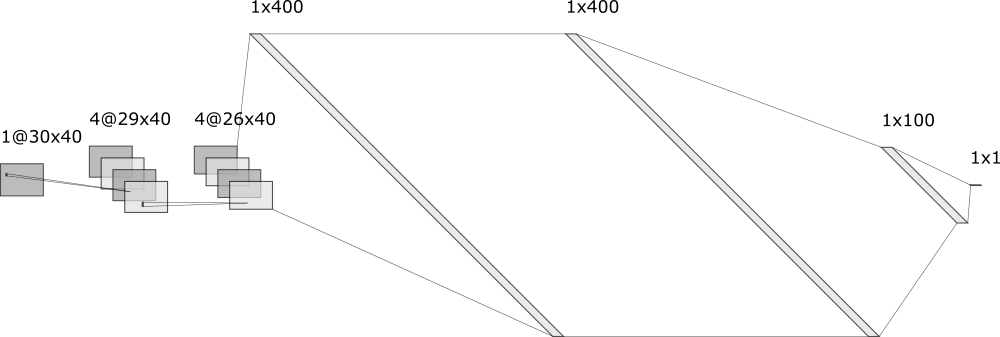
\includegraphics[width=0.7\textwidth]{figures/regression/fourier/cnn/fourier_conv_layout.png} 
    \caption[Layout of LEFD CNN]{
        Architecture of the convolutional neural network used for predicting the activation barrier from fourier coefficients.
    }
    \label{fig:cnn-architecture}
\end{figure}

In first network architectures, overfitting was a mayor problem.
With regularization and other techniques the issue of overfitting could be reduced.
What became clear pretty early in the tests was that convolution layers did not improve prediction accuracy as expected.
When testing different filter configurations, the network performed best the smaller the filters got, and the fewer convolution layers were used.
In the end, the best performing Convolutional Neural Network found had two Convolution Steps with a filter size of $2 \times 1$ for the first layer, and a filter size
of $4 \times 1$ for the second layer Figure~\ref{fig:cnn-architecture}.
After the convolution layers 3 fully connected layers and the output layer followed.
Dropout and batch normalization layers were added in between to reduce overfitting.
The prediction accuracy of the CNN was similar yet slightly worse than the prediction accuracy achieved on autocorrelation features \cite{friederich_dos}.
The best CNN achieved a mean squared error over all test examples of $MAE=1.36 kcal/mol$ and a coefficient of determination of $r^2=0.84$ \ref{fig:fourier_cnn}.
In comparison, the best neural network of \cite{friederich_dos} achieved a prediction accuracy of $MAE=1.12 kcal/mol$ and $r^2=0.845$.

Since the space of possible network configurations is highly irregular, there is likely a network configuration using convolution layers 
that performs better than the one found here.
However all the tests performed were indicating that densely connected layers would achieve similar or higher accuracy.
The idea of convolution layers was therefore dropped early on, and instead the focus was shifted to optimizing a fully-connected architecture.
\\ 

\begin{figure}[!htb]
    \minipage{0.1\textwidth}
    \endminipage\hfill
    \minipage{0.4\textwidth}
      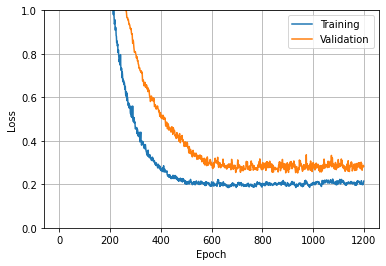
\includegraphics[width=1.0\textwidth]{figures/regression/fourier/cnn/lossCNN.png}
    \endminipage\hfill
    \minipage{0.4\textwidth}
      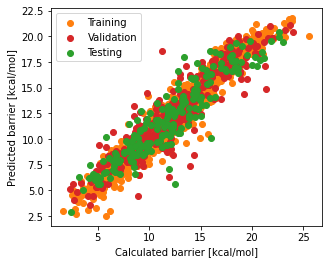
\includegraphics[width=1.0\textwidth]{figures/regression/fourier/cnn/scatterCNN.png}
    \endminipage\hfill
    \minipage{0.1\textwidth}
    \endminipage
    \caption[CNN trained on LEFD features]{
        Loss while training the CNN. The jitter in the training loss during convergence is likely caused by the dropout layers. 
        The optimization goal was minimizing the mean squared error. 
        Training was performed on 80\% of the data.
        On the right are the predictions of the activation barrier in comparison to the real values ($MAE=1.36$, $r^2=0.84$).
    }
    \label{fig:fourier_cnn}
\end{figure}

Since \cite{friederich_dos} has shown that similar accuracy to the convolution approach can be achieved by learning from autocorrelation features,
the next idea was to use a transfer learning approach.
In a first step, the network was trained to predict the autocorrelation features computed in \cite{friederich_dos}.
In a second step, the network is then extended with additional layers to learn to predict the activation barrier \ref{fig:transferlearn}.
The hope was that teaching the network about autocorrelation features, the model would learn to recognize relevant properties of a catalyst.
In a second step, the entire network would then be trained to adapt specifically to the activation barrier.

\begin{figure} [h]
    \centering
    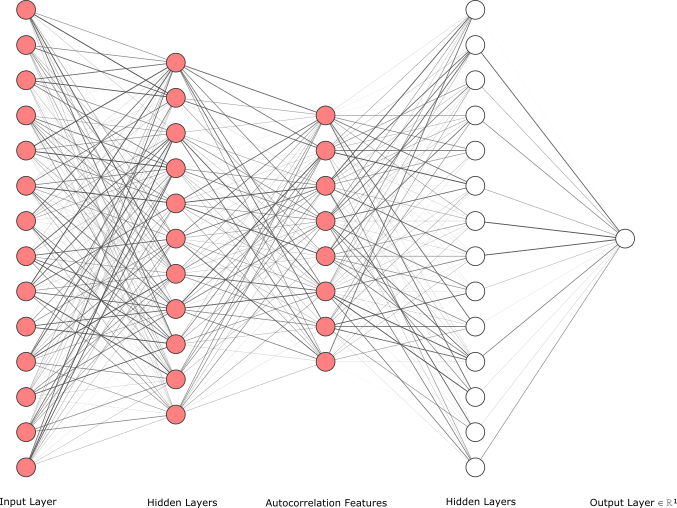
\includegraphics[width=0.7\textwidth]{figures/regression/fourier/nn.png} 
    \caption[Transfer learning model]{Illustration of the transfer learning approach.
        In red the original model predicting autocorrelation features from the input is illustrated.
        In white the second part of the network, predicting the activation barrier from the autocorrelation features, is illustrated.
        Different sizes and amounts of hidden layers were tested. Here, single hidden layers are shown for illustration purposes.
    }
    \label{fig:transferlearn}
\end{figure}

Since the convolutional approach did not seem to improve results, a fully connected architecture predicting autocorrelation features from fourier coefficients 
was used.
Since there were 30 autocorrelation features used, the last layer of the network had a size of 30.
Findings about good hyperparameter, such as layer size, regularization and dropout rates, could be partly reused from the convolution step.
In the end, a network that predicted the 30 independent autocorrelation features was found.
The network was able to predict some autocorrelation with very high accuracy. Specifically, the $T$ features and $I$ features were
predicted with an accuracy of $r^2 > 0.98$. 
Other features, such as $Z$ features, were lacking behind in accuracy, with the network only being able to reach accuracy of $r^2<0.96$ for some features.
The features the network was able to approximate well were also less important to the network found in \cite{friederich_dos}, while the features 
the network performed poorly on were the more important features \ref{fig:transfer_result}.

\begin{figure}[h]
    \minipage{0.32\textwidth}
      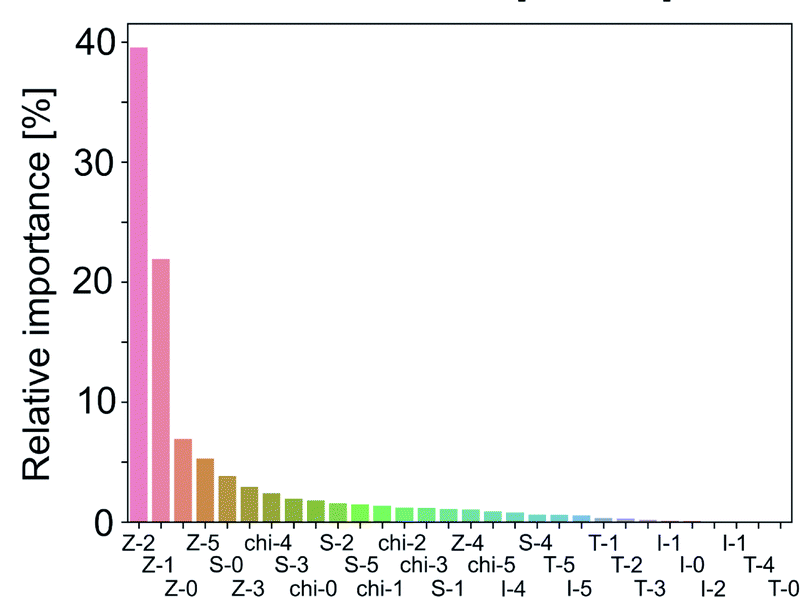
\includegraphics[width=1.0\textwidth]{figures/regression/fourier/importance_map.png}
    \endminipage\hfill
    \minipage{0.32\textwidth}
      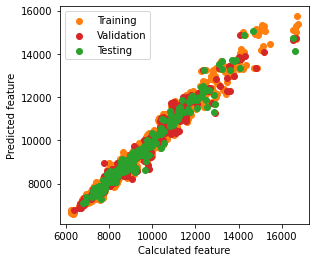
\includegraphics[width=1.0\textwidth]{figures/regression/fourier/transfer/scatterZ2.png}
    \endminipage
    \minipage{0.32\textwidth}
      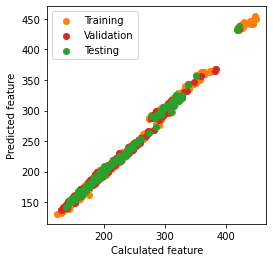
\includegraphics[width=1.0\textwidth]{figures/regression/fourier/transfer/scatterT0.png}
    \endminipage
    \caption[Prediction of autocorrelation features from LEFD]{
    Left: Importance of features for the neural networks discussed in \cite{friederich_dos}.
    Middle: Prediction of Z-2 features from fourier features.
    Right: Prediction of T-0 features from fourier features. 
    The network was trained on 80\% of the data points.
    }
    \label{fig:transfer_result}
\end{figure}

After the network predicting the autocorrelation features was trained, the transfer learning was started.
The last layers of model were removed, and replaced with newly initialized layers.
These newly added layers have an output size of 1 to allow for prediction of the activation barrier.
The best configuration found kept the first 3 layers of the original network, and then added 3 additional hidden layers and one output layer.
Regularization and normalization was used for some of the layers.
The model was then trained again with fourier coefficients as input and activation barriers as output.
Compared the convolution approach, the network took longer to converge and overall regression accuracy improved.
The network achieved a $r^2=0.874$ and a $MAE=1.139 kcal/mol$ when trained on 80\% of the data Figure~\ref{fig:transfer_final}.

\begin{figure}[!htb]
    \minipage{0.3333\textwidth}
      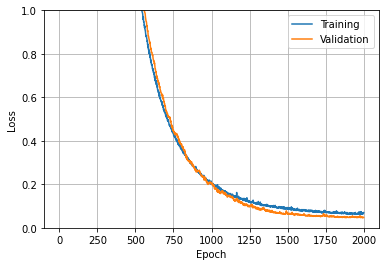
\includegraphics[width=1.0\textwidth]{figures/regression/fourier/transfer/lossTransferAutocor.png}
    \endminipage\hfill
    \minipage{0.3333\textwidth}
      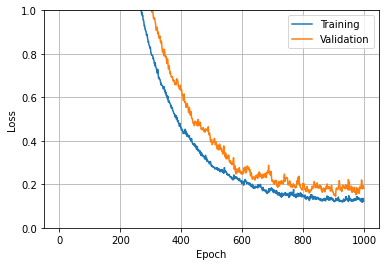
\includegraphics[width=1.0\textwidth]{figures/regression/fourier/transfer/lossTransferFull.png}
    \endminipage\hfill
    \minipage{0.3333\textwidth}
      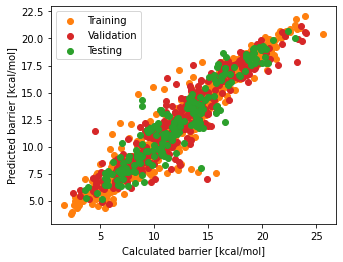
\includegraphics[width=1.0\textwidth]{figures/regression/fourier/transfer/scatterTransferFull.png}
    \endminipage
    \caption[LEFD transfer learning]{
    Loss of the network being trained to predict autocorrelation features (right).
    The adapted network is then trained again to predict the activation barrier. The loss function in the middle shows the second training.
    The prediction accuracy has slight improved (right).  
    }
    \label{fig:transfer_final}
\end{figure}

In an attempt to find a better network architecture, a hyperparameter optimization was performed.
Hyperparameter optimization is a way of finding good hyperparameter for the underlying problem.
A searchspace need to be defined manually first, an optimization algorithm is then run to find good parameters within the search space.
Generally a bigger search space mean longer computation time for the hyperparameter algorithm.
The search space here was limited by the findings of manual hyperparamter tuning.
Notable optimization values given to the hyperparamter tuner were the number of convolution layers, 
the number and size of fully connected layers, the regularization rate of these layers, and the dropout rate for the layers.


\begin{figure}[!htb]
    \minipage{0.3333\textwidth}
      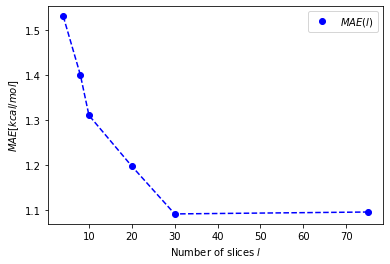
\includegraphics[width=1.0\textwidth]{figures/regression/fourier/mae_layer.png}
    \endminipage\hfill
    \minipage{0.3333\textwidth}
      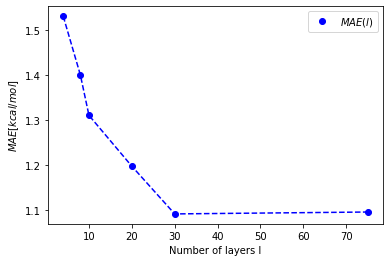
\includegraphics[width=1.0\textwidth]{figures/regression/fourier/r2_layer.png}
    \endminipage\hfill
    \minipage{0.3333\textwidth}
      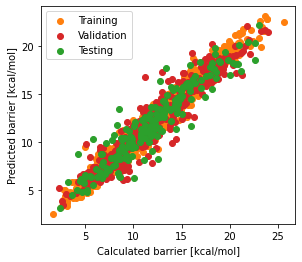
\includegraphics[width=1.0\textwidth]{figures/regression/fourier/scatterHyperparam.png}
    \endminipage
    \caption[Evaluation of LEFD models]{
    The $r^2$ values and $MAE$ for different layer heights.
    For all layer heights a separate hyperparameter optimization wa run, resulting in different network architectures.
    All networks are trained using 80\% on the data. The $r^2$ scores and $MAE$ were evaluated later using a test dataset.
    On the right the prediction of the best performing network found in the hyperparameter optimization step is plotted.
    }
    \label{fig:fourier_final}
\end{figure}


In addition, multiple hyperparameter optimizations were performed for different layer heights $l$.
Since the layer heigh also changes the input size of the neural network, an assumption about the 
architecture across different layer heights is not feasible.
For ever layer height a separate hyperparamter optimization was run Figure~\ref{fig:fourier_final}.
The best hyperparameters found for every input size vary substantially.
The best network achieved an accuracy of $MAE=1.096 kcal/mol$ and $r^2=0.882$ on a training fraction of 80\%.
It was trained on features generated from a layer height of $0.2$, resulting in a total of $75$ layers.

After a certain layer height the prediction accuracy seems to no longer improve.
The step from 30 to 75 layers does not change the accuracy significancy, while more than doubling input size.
The improvement in accuracy from 30 to 75 layers is so small that it might be an artifact of the 
randomness of training, and does not necessarily mean that the network is able to learn better from the higher amount of layers.

The process shows that performing regression on fourier features is possible.
The accuracy however is not significantly higher than the accuracy achieved on graph convolutions.
Since the goal of this thesis is to learn from the 3D structure of the molecule, the similar performance to networks trained on autocorrelation features
might indicate that the information learned from the 3D structure is limited.
This assumption is further validated by the fact that the transfer learning approach that 
tries to eliminate spacial information about the element in the middle of the network, achieves similar accuracy to the 
network trained on features that do not include any information about the 3D structure.

In an effort to improve prediction accuracy, a different feature extractor, SNAP, was developed.

\section{Regression on SNAP features}
\label{sec:Evaluation:snap}

Similar to the feature space for fourier coefficients, the shape of the SNAP feature space is determined by two factors.
The first is the number of different species in the dataset.
The second is the resolution of the encoding defined by $n_{max}$ and $l_{max}$.

Other hyperparameters, such as the choice of radial basis functions, might influence the prediction accuracy further.

The number of radial basis functions $n_{max}$ and the maximum degree of spherical harmonics $l_{max}$ do both influence
the input dimension.
The ideal network architecture for different values will depend on the choice of these values.
The higher the degree of the spherical harmonics and radial basis functions, the more precise the element can be described. %TODO: The element or the space?
The choice of $n_{max}$ and $l_{max}$ will also determine the accuracy when trying to interpret the predictions of the model later on.

Hyperparameter analysis was performed on different combinations of $n_{max}$, $l_{max}$.
Since hyperparameter optimization is very computationally expensive, taking up to multiple days on modern high-performance 
server hardware, the number of combinations that could be explored is limited.

SNAP features are not fully rotationally invariant.
In order to allow the model to learn about the different possible rotations of the molecule, data augmentation was used.

During the hyperparameter optimizations, 20 evenly spaced rotations of the molecule along the $z$-Axis were used.
The features for all of the 20 rotations was then fed into the model.
Tests with different augmentation steps showed that 20 augmentations seemed to be a good balance between 
accuracy and training speed.
Since the size of training examples rises linearly with the number of data augmentations,
high numbers of augmentations will drastically decrease training speeds.
This will in effect also reduce the speed of hyperparameter optimization.

Later on the architectures found by the hyperparameter optimizer with 20 data augmentation steps, 
models with higher data augmentation steps were trained in an effort to improve prediction accuracy further.

\subsection{Convolution Neural Network}

Similar to the features generated by EFD, the output of SNAP can be shaped into a feature matrix again.
Here, each layer will correspond to one species of atoms.
Since the dataset the model is trained on consists of 12 different species of atoms, the feature matrix will have a height of 12.
Each row will then contain the coefficients describing the density of one species around the iridium center.
Depending on the choice of $n_{max}$ and $l_{max}$, the number of coefficients for each species will change.

Since a coefficient of the $k$-th row will correspond to $c^k_{nlm}$, meaning every coefficient in the same colum has the same spacial meaning just for a different species,
a convolutional neural network was the first idea to reduce the size of the input space and allow the network to learn structure in the input data.

Since not every molecule in the dataset consists of every atom, the input matrix will generally be sparse.
Rows that correspond to atoms not in the dataset will be filled with 0.
A filter that learns the general structure of the space and that is moved over the different species, therefore 
being able to ignore sparse inputs seemed to be a good choice.

Using a hyperparameter optimization to find the ideal filter size and number of convolution layers however showed
the a fully connected approach reaches higher accuracy than convolutional layers.
The hyperparameter optimizer not only gravitated towards a small amount of filters, but also towards 
the smallest possible filter size allowed in the hyperparameter space.

In further optimization the idea of convolution layers was therefore dropped in favour of fully connected layers.

If in the future the $n_{max}$ and $l_{max}$ parameters or the number of species are increased drastically, 
convolutional layers might become relevant again.

\subsection{Fully connected neural network}

In a next step, hyperparameter optimization was focused on fully connected layers.
For different combinations of $n_{max}$ and $l_{max}$ hyperparameter optimizations were run.

The hyperparameter optimizer was allowed to choose between 1 to 6 hidden layers.
For each layer, the number of neurons, regularization rate and dropout rate could be chosen by the optimizer.
Additionally, the optimizer had the option to add a batch normalization layer after each of the layers.
The layers were then finished off with one neuron fully connected to the last hidden layer.

The activation function for each of the layer was fixed to Relu activations.

Using the Hyperband Optimizer, the configurations discussed in the following sections were found.

\paragraph{Feature size}
The expectation was that the more accurate the density space would be described, the higher the prediction accuracy would be.
However after a full hyperparameter optimization on a variety of combinations of $n_{max}$ and $l_{max}$,
the differences in accuracy were not as significant as expected.
While increasing the number of $n_{max}$ coefficients seemed to increase the prediction accuracy,
increasing the number of spherical harmonics $l_{max}$ did not play a significant role in prediction accuracy Figure~\ref{fig:snap_hyperparameter}.
Highest prediction accuracies where achieved by networks performing regression on features generated with $n_{max} > 6$.

The interpretation here is that distance to the metal center plays an important role to predicting the activation
barriers in the dataset, while the location seems to be less important.

Since hyperparameter searches for are very costly, taking up multiple days on modern day cloud-computing hardware,
hyperparameter analysis was run to an $l_{max} = 9$.
Significantly increasing $n_{max}$ might further improve prediction accuracy.

%TODO: Redo with actual values
\begin{figure}[!htb]
  \minipage{0.3333\textwidth}
    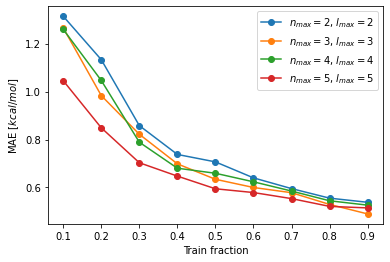
\includegraphics[width=1.0\textwidth]{figures/regression/snap/fixnl.png}
  \endminipage\hfill
  \minipage{0.3333\textwidth}
    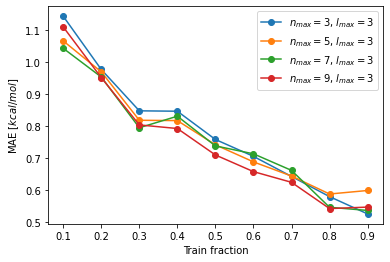
\includegraphics[width=1.0\textwidth]{figures/regression/snap/fixl.png}
  \endminipage\hfill
  \minipage{0.3333\textwidth}
    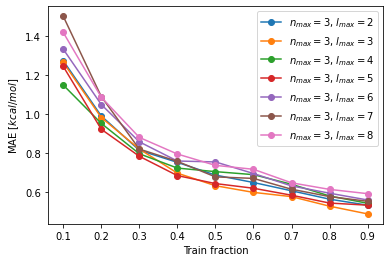
\includegraphics[width=1.0\textwidth]{figures/regression/snap/fixn.png}
  \endminipage
  \caption[Learning curves for different SNAP resolutions]{
  Networks for SNAP features trained on different train fractions.
  All networks were trained on the hyperparameters found for the corresponding $n_{max}$ and $l_{max}$.
  Networks were trained with 10 data augmentation steps and a cutoff radius of $12 \AA$.
  Hyperparameter search was run on a training split of 80\%.
  }
  \label{fig:snap_hyperparameter}
\end{figure}

\paragraph{Cutoff sphere}
All hyperparameter searches were run with with a cutoff radius $r_{cut} = 20 \AA$.
This cutoff sphere is large enough to fully fit every element of the dataset into it.
However, due to the nature of the radial basis functions used, the resolution of atoms 
further away from the center will decrease.
To test the influence of the cutoff radius on the prediction, 
networks were trained on features generated with different cutoff radii.
The network architecture was based on the hyperparameter optimization performed earlier.
Since the networks architecture is not fully optimized to the cutoff radii, the prediction accuracies
of the networks were not up the levels found in fully hyperparameter optimized networks.
However the assumption was made that good values for $r_{cut}$ on these not fully optimized architectures 
will also translate to good values under fully hyperparameter optimized networks.
This significantly decreased the number of hyperparameter search needed.
Since hyperparameter search will take multiple days to finish, while networks with known hyperparameters
can be trained in a matter of minutes, this meant a significant speedup.


For every configuration of $n_{max}$ and $l_{max}$, a networks were trained for a variety 
of tests splits and data augmentation steps.
These networks were then evaluated by their performance with respect to the cutoff radius.

Up to a cutoff radius of $10 \AA$, the mean network performance improved. %TODO: Rich
At a training fraction of 80\%, the mean classification error among 
all networks decreased from $0.889 kcal/mol$ for a cutoff radius of $5 \AA$ to 
$0.801 kcal/mol$ for a cutoff radius of $10 \AA$.
From there however, increasing the cutoff radius did not improve the accuracy further.
This lead to the hypothesis that atoms closer to the metal center are more important to the activation barrier than atoms further away from the center.
This hypothesis could also explain the slight increase in prediction error when further increasing the cutoff radius.
Since the resolution of the feature space is limited, increasing the cutoff radius will decrease the accuracy 
with which the inner atoms are described in the features, which might have caused a decrease in prediction accuracy.

To verify this hypothesis, a second experiment was run.
Here, all atoms outside a cutoff sphere were removed from the element before passing it on to the encoder.
The atoms were then encoded with a cutoff radius $2 \AA$ higher than the cutoff sphere to allow for a proper 
encoding of atoms just inside the cutoff sphere.
The networks were once again trained with the hyperparameters found in the initial hyperparameter analysis.
The training was run for cutoff spheres of $2\AA, 4\AA, 6\AA, 10\AA, 15\AA, 20\AA$ resulting in $r_{cut}$ 
of $4\AA, 6\AA, 8\AA, 12\AA, 17\AA, 22\AA$.
For $r_{cut}=4$, no prediction was possible and the networks just predicted the mean of the data.
This was to be expected since at this cutoff radius, only 20\% of the elements are encoded into the features.
However for $r_{cut}=8$ the mean MAE over all networks trained on 80\% of the data was at $MAE = 0.834 kcal/mol$. 
For $r_{cut} = 8$, resulting in a cutoff sphere of $6 \AA$, 96\% of the atoms are included in the data. 
The remaining 4\% fall outside of the cutoff sphere and are ignored. 

For $r_{cut}=12$ the mean MAE over all networks trained on 80\% of the data was at $MAE = 0.836 kcal/mol$. 
At this cutoff radius, 100\% of the atoms are included in the data.
While this accuracy is marginally higher, the difference is so small that is could 
simply be explained by the optimizer falling into different local minima compared to $r_{cut}=8$. 

This lead to the conclusion that, while all atoms in the dataset seem to have an effect on the prediction,
choosing a tight $r_{cut}$ achieves the best prediction accuracies.
When looking at the nature of the encoding, this intuition is verified.
Empty space that is indirectly included into the enocoders features.
Since the encoder will try to encode a density of 0 in these regions,
the features need to be chosen accordingly.
This means the features to encode empty space will compete with the features encoding
actual information about the molecule.
The less empty space needs to be encoded, the more accurate actual density can be represented.
From now on, all cutoff radii will therefore be chosen at $r_{cut} = 12 \AA$.

\begin{figure}[!htb]
  \minipage{0.5\textwidth}
    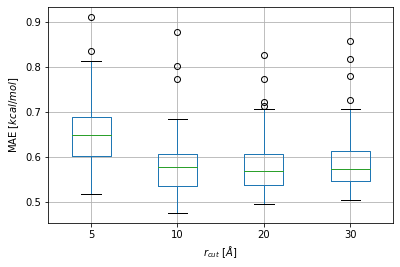
\includegraphics[width=1.0\textwidth]{figures/regression/snap/cut-all.png} %TODO: REPLACE!!!!
  \endminipage\hfill
  \minipage{0.5\textwidth}
    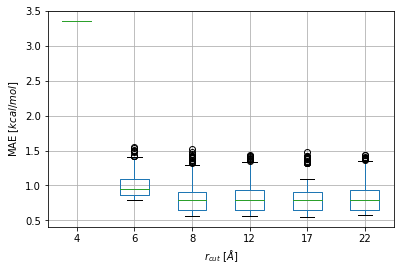
\includegraphics[width=1.0\textwidth]{figures/regression/snap/cut-sphere.png}
  \endminipage\hfill
  \caption[Comparison of SNAP cutoff radii]{
  Networks trained on different cutoff radii. All networks are trained on a train fraction of 80\%.
  On the left a variety of networks with different $n_{max}, l_{max}$ trained on a test train split of 80\% is shown.
  On the right are networks trained with a cutoff sphere outside of which all atoms are removed. 
  The radius of the cutoff sphere is $r_{cut}-2$.  
 }
  \label{fig:snap_hyperparameter}
\end{figure}


\paragraph{Sensitivity to rotation}
Since SNAP features are not fully rotationally invariant, the networks ability to abstract rotation from the input is crucial.
In order to teach the network about the possible rotations of an element, 
the element is augmented by rotating it around the remaining axis of freedom, the $z$ axis.
For every augmentation step, the rotated element is added to the training data.
Tests with different augmentation steps were performed.
All networks were trained on the previously found hyperparameters.
The augmentation steps ranged from 5 evenly spaced rotations to 100 evenly spaced rotations.
Both the training and the test data was augmented to allow for learning from the augmented data
as well as to validate if the network was actually able to abstract away rotations.

Even with only 5 data augmentation steps the networks achieved a mean prediction error of $MAE = 0.584 kcal/mol$.
The mean error over all networks decreased up to 40 augmentation steps.
After 40 augmentation steps no further decrease in mean prediction error was observed.% ~\ref{fig:snap_roation_out}.
For networks with higher data augmentation steps, the stability of the networks when trained on small train splits was higher.

When looking a networks prediction over 360 different rotations, networks trained with higher data augmentation 
are significantly more stable to rotation than networks trained on a smaller number of of rotations \ref{fig:snap_roation}.
When comparing a network trained on 20 rotations to a network trained on just 5 rotations,
the difference becomes clear.
For the network trained on 5 rotations the prediction accuracy is high for rotations included in the training data.
For rotations not in the training data, the prediction diverges significantly, indicating the inability of the network to abstract awy rotation.

For the network trained on 20 rotations, the divergence is very limited.
However in some cases, while the overall prediction accuracy is decreased for the network trained on 
more data augmentations, the accuracy for some rotations is more precise on the network trained on a lower number of augmentations.
Since there is no way of knowing which rotation is the one with the closest to real prediction, in 
a real world application the network trained on a higher data augmentation size is preferable.

Between a augmentation size of 20 to 30, the networks ability to better abstract away rotation is stagnant.
Augmenting the data by 20 to 30 steps therefore seems sufficient to teach the network about all possible rotations.
Interestingly, for some networks while the ability to abstract away rotation no longer increases after 20 augmentation 
steps, the overall performance increases slightly, especially for small training splits.

One hypothesis here would be that the higher number of training data that comes with a bigger number of data augmentations
helps the network to learn about the general structure of catalyst molecules.
While the different rotations of the molecule do not include any new data, they still contain the 
general shape of a catalyst.
This might help the network learn about the general topology of the input data.

Transfer learning might utilize this property in further improvements.
In the future the test error might be improved by creating a second dataset with a variety of different catalysts molecules.
Due to the combinatorial approach in which molecules surrounding Vaska's complex can be generated, 
creating datasets with a large number catalyst molecules is relatively simple.
The problem comes with calculating their activation barrier.
The key advantage of a transfer learning approach to pre-train the model is that the activation barrier of the extended dataset does not have to be computed.
Instead, properties related to the activation barrier that can be easily computed from the molecules structure are generated.
In a first step, the network would then be taught to predict these east to compute features.

In a second step, the networks topology would be slightly adapted to perform single values regression.
However, the weights and biases will not be changed.
The network is then trained again on the small dataset for which the activation barrier is known.

This approach might help the network to gain more knowledge about the general structure of a catalyst molecule,
and thus reduce overfitting.
The hope is that with this approach the prediction accuracy will improve again.

If this hypothesis holds true will have to be explored in further experiments.


\begin{figure}[!htb]
  \centering
  \minipage{0.4\textwidth}
    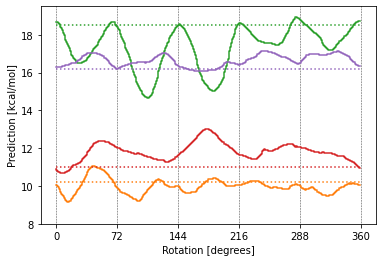
\includegraphics[width=1.0\textwidth]{figures/regression/snap/aug-5steps-30per.png}
  \endminipage\hfill
  \minipage{0.4\textwidth}
  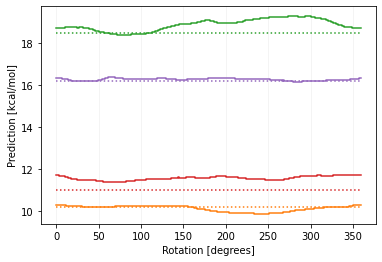
\includegraphics[width=1.0\textwidth]{figures/regression/snap/aug-30steps-30per.png}
  \endminipage
  %\hfill  
  %\minipage{0.3333\textwidth}
  %  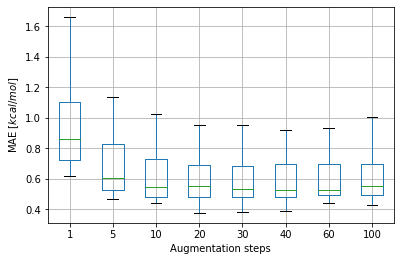
\includegraphics[width=1.0\textwidth]{figures/regression/snap/augmentation.png}
  %\endminipage\hfill
  \caption[Evaluation of SNAP rotational invariance]{
  The predictions for a network on SNAP features for $n_{max}=9, l_{max}=3$ trained with 5 data augmentation steps (left) 
  and 20 augmentation steps (right) for 4 randomly selected samples. 
  The continuos line is the prediction of the network, the dotted line is the calculated barrier.
  The networks were trained on a train split of 70\%.
  %On the right are the results for multiple models trained on different augmentation steps.
  %All networks are trained on the same network architecture, at different train fractions.
  }
  \label{fig:snap_roation}

\end{figure}


\paragraph{Results}

With the data learned from the extensive hyperparameter and input space exploration, a final hyperparameter
optimization was performed.
This hyperparameter optimization took into account the values discussed previously, and therefore was run on 
features  generated with $8 \leq n_{max} \leq 9, 3 \leq l_{max} \leq 4, r_{cut}=12$.
30 data augmentation steps were passed to the hyperparameter optimizer.
Hyperparameter optimization was run on a train fraction of 80\% of the dataset.
This time, the hyperparameter space was increased slightly to allow the optimizer
to choose from up to 10 hidden layers, each with a maximum amount of 1000 neurons.


\begin{figure}[!htb]
  \minipage{0.5\textwidth}
    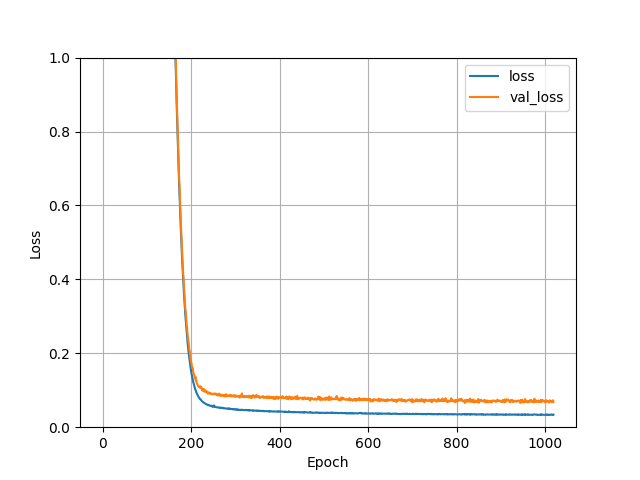
\includegraphics[width=1.0\textwidth]{figures/regression/snap/loss_8-4.png}
  \endminipage\hfill
  \minipage{0.5\textwidth}
  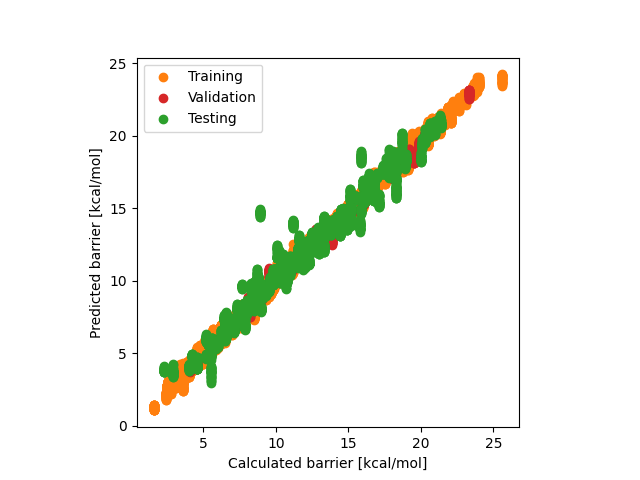
\includegraphics[width=1.0\textwidth]{figures/regression/snap/scatter_8-4.png}
  \endminipage\hfill  
  \caption[Best performing model on SNAP features]{
    Loss of the best performing model on SNAP features on the left. 
    The loss function used is mean squared error.
    Predictions of the model trained on a training fraction of 80\% on the right. 
    For every sample, 30 data augmentation steps are used. This makes some samples appear like small vertical lines.
  }
  \label{fig:snap_roation}

\end{figure}


Even with slight variations in prediction accuracy due to rotation, the overall results of regression performed on SNAP features is still promising.
All models found during hyperparameter optimization for different $n_{max}, l_{max}$ were able to predict the reaction barrier with higher accuracies in the
range of the best models found so far.
With the best models for $n_{max}=8, l_{max}=4$ achieving accuracies of $MAE=0.539 kcal/mol$ and $r^2=0.960$. %TODO: Verbessern

The network has a total of 7 hidden layers.
Dropout and batch normalization layers are added in between \ref{fig:architectures}.

Compared to other modes of encoding the data, SNAP seems to be especially susceptible to outliers.
For all models, the regression accuracy is heavily influenced by a small number of samples with poor precision.
Since the split between training and test data is random, the overall accuracy of the model is 
heavily influenced by the selection of samples in the test data.
The same holds true for the randomness between training and validation data.

Improving the networks stability to outliers could further increase regression accuracy.


\section{Comparison}
\label{sec:Evaluation:Comparison}

The neural networks proposed here were able to predict the activation barriers with high accuracies.
The reference values to the networks was given by \cite{friederich_dos}, where different Machine Learning 
approaches to the regression problem were introduced.
While the dataset was the same in \cite{friederich_dos}, the features extracted from the molecules were different.
The comparison of the results from \citetitle*{friederich_dos} and this thesis is therefore more 
a comparison of feature extractors, and not a comparison of machine learning methods or network architectures.

Their best neural network trained on 80\% of the data achieved a prediction accuracy of $MAE = 1.12 kcal/mol$ and a 
coefficient of determination of $r^2 = 0.845$.
The neural network was 4 layers deep and trained on their autocorrelation features.
Autocorrelation features extract features from a graph representation of the chemical structure, but neglect the 
3D structure of the molecule \cite{friederich_dos}.
The best prediction accuracy was however in a yet unreleased paper by  a graph convolution neural network (GNN) on 
a graph structure of the molecule.
It achieved an accuracy of $MAE = 0.571 kcal/mol$ and $r^2=0.964$.
These are the highest accuracies achieved on this dataset yet.
While this was the state-of-the-art  to compare the models in this thesis to, the main objective was not to beat these numbers.
The goal was rather to achieve similar performance with a feature descriptor that allowed for a mapping back from feature space to 3D space.
This allows for an extensive interpretation of the results, which is impossible with current features.
The SNAP features however not only allow for this analysis, but are also able to beat the accuracy of GNN models.
Another important metric is the performance of the networks for different sizes of training data.
The models performance will therefore be compared by their accuracy for different test split sizes.
\\
The first approach regression was using LEFD features.
When training on 80\% of LEFD features, the best neural network achieved an accuracy of $MAE = 1.096 kcal/mol$ and $r^2=0.882$.
While the accuracy is slightly higher than the best neural network in \cite{friederich_dos}, it still falls short 
of both the GNN and other machine learning models.
At lower train fractions the accuracy decreases faster than other methods.
Interestingly, the accuracy of the model is very similar to the accuracy achieved by the neural network trained on autocorrelation 
features.
Additionally the autocorrelation features could be approximated from the LEFD features reasonably well.
This could indicate that LEFD features and autocorrelation features describe
similar information about the element that is relevant to the activation barrier. %TODO: Stimmt eher nicht, andere ML methoden sid ja besser
\\
The best models trained on SNAP features were able to achieve accuracies of $0.0.539 kcal/mol$.
While the final accuracies are heavily dominated by outliers, models trained on SNAP features were consistently
able to achieve accuracies better than the best models trained on other features.
Another interesting property of models trained on SNAP is their ability to perform well with small amounts 
of training data.
Even with training fractions well below 50\% of the data, the network still achieved good accuracies.
At train fraction below $10\%$ the accuracy drastically decreases.

The biggest problem with SNAP features so far seems to be their sensitivity to outliers.
While the majority of the elements in the dataset is predicted with very high accuracy, 
there are some outlier with very poor performance.
Depending on the application of the network, a network with a lower overall accuracy 
that is less susceptible to outliers might be better suited.

\begin{figure}[!htb]
  \minipage{0.5\textwidth}
    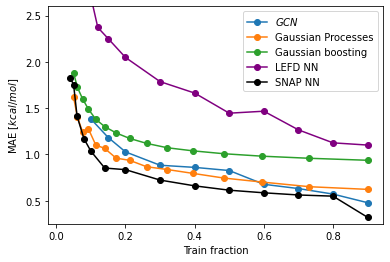
\includegraphics[width=1.0\textwidth]{figures/regression/mae-compare.png}
  \endminipage\hfill
  \minipage{0.5\textwidth}
  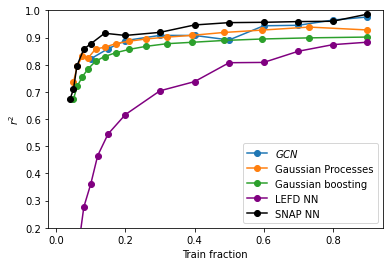
\includegraphics[width=1.0\textwidth]{figures/regression/r2-compare.png}
  \endminipage\hfill  
  \caption[Comparison of learning curves]{
    Learning curves of different machine learning methods on the same dataset.
    Gaussian Process and Gaussian Boosting models were proposed in \cite{friederich_dos}.
    The GCN is a unpublished result by \citeauthor{friederich_dos}.
    Other results are taken from \cite{friederich_dos}.
  }
  \label{fig:snap_roation}

\end{figure}



\section{Explaining the prediction}

Traditionally neural networks are seen as a black-box approach to data analysis.
The network is given a set of training data and trained to fit onto the data,
the internals of the network however are set by the optimization algorithm.

This makes it hard to interpret the origin of predictions of the network.
Network explaining methods aim to help to understand the origin of a prediction in the features.
Translating the features back into chemical space can help to better understand 
the elements in the dataset and might give intuitions on how elements have to be adapted in order to change their activation barrier.

Since SNAP features achieved significantly higher prediction accuracies,
this analysis was focused on SNAP features only.

\subsection{SHAP}

The first approach to explaining the feature space was using the SHAP feature explainer.
SHAP offers analysis of the influence of different features to the final prediction \cite{NIPS2017_7062}.
This allows get an intuition on how different species influence the activation barrier.

When using SHAP values on the model, the contribution of each feature to the current prediction can be observed.
The values generated by SHAP are a matrix the sitze of the input to the network.
Summing over all SHAP values for one sample will give the prediction of that sample.
When labels for the features are  known, SHAP is often visualized as as features pushing in opposite direction with different force 
to achieve the prediction of the model.
The SHAP values will not correspond to the activation barrier directly,
but rather to the scaled activation barrier used to train the network.

Scaling issues make the interpretation of the SHAP values difficult.
Thinking back to the main objectives of SNAP, being able to convert the features back into 
a 3D density was one of the main objectives.
While the formula describing the density space could be used to transform the SHAP values 
into a 3D density, it is unclear how the density generated by SHAP would have to be interpreted.

Due to the nature of the SNAP encoder, a negative $c_{nlm}^Z$ values does not automatically 
describe a negative density.
This means a negative SHAP values for an element does not equate reduction in density
at a point in space.
In order to get information about the 3D space surrounding the atom, the SHAP values would have to be converted back into 3D density space.
This is a problem since the features indicate their influence on the prediction, but do not necessarily correspond 
to the 3D spacial encoding.
The SHAP values therefore are in the scale of the activation barrier.
When converting SHAP values back to 3D, it is unclear how these scaling issues would 
affect the result. 
This uncertainty prohibits a interpretation of the density space.
Examining the density space for it's influence on the prediction is only possible if the scaling
issues can be solved.
Since the scaling issues did not seem to be easily solvable, a second attempt to explain the origin of the prediction
was run using a gradient based method.

The information that can be extracted from SHAP values therefore is limited to feature space.

In the case of Figure~\ref{fig:shap}, the features corresponding to bromine and arsenic seem to decrease the barrier.
Interestingly the features encoding the absence of phosphorus seem to increase the barrier.

A good sign that the values have some validity is that Iridium never influences the barrier.
Since iridium is present exactly once in all elements, it should not carry any information about the barrier,
and therefore not influence the prediction at all.

SHAP allows to get some intuition of the element and how it is atoms influence the barrier.
However for now the information we can gain is limited to a global representation of the element.

If the scaling issues can be resolved, SHAP might offer further and detailed insight into how different parts of an element influence it's activation barrier.

\begin{figure}
    \centering
    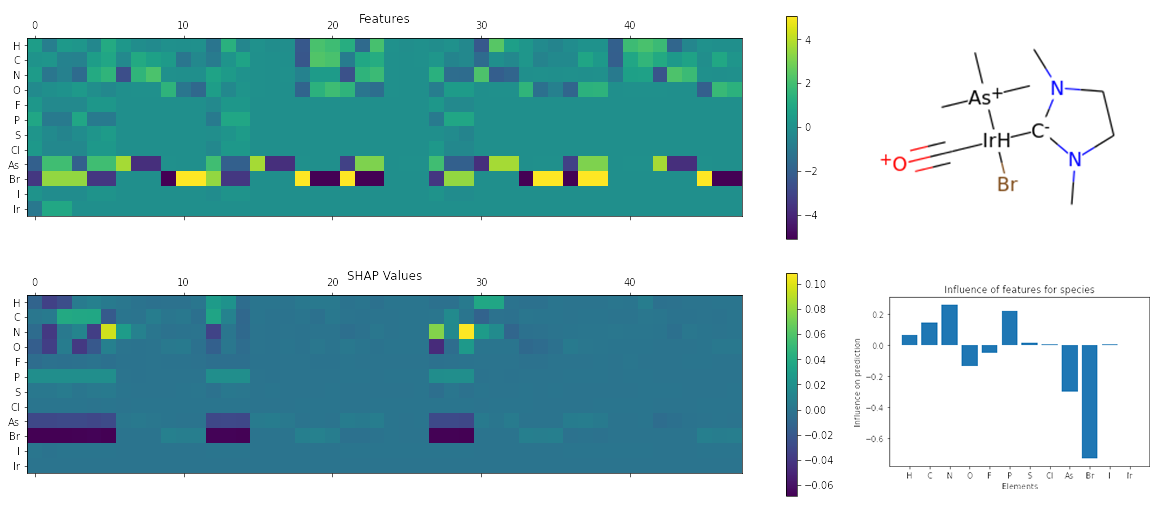
\includegraphics[width=0.9\textwidth]{figures/evaluation/SHAP.png}
    \caption[SHAP values]{
        Features($n_{max}=l_{max}=3, r_{cut}=12$) generated by the element on the right and the corresponding SHAP values.
        The element has a calculated barrier of $10.2 kcal/mol$.
        Because the activation barriers are scaled to achieve higher prediction accuracies,
        the values our network predicts is $-0.494$ which scaled back results in a predicted activation 
        barrier of $9.83 kcal/mol$.
     }
    \label{fig:shap}
  \end{figure}
  



\subsection{Gradient explainer}

On  of the interesting properties of neural networks predicting the activation barrier from the 3D shape is 
that an intuition on how changes in 3D space will influence the activation barrier can be gained.

In contrast to SHAP values that explain the contribution of a feature to the prediction of a model, 
computing the gradient of a model will give an idea on how changing a certain feature will affect the prediction of the model.

Let the model $N$ be a function from feature space $\mathbb{R}^n =: \mathbb{S}$ to the activation barrier of the element $\mathbb{R}^+_0$.
Since a function from density space $\mathbb{D}$ to feature space $\mathbb{S}$ can be defined,
a mapping from density space to the activation barrier can be found.
$$ \Psi : \mathbb{D} \to \mathbb{S} \to \mathbb{R}^+_0, e \mapsto \Psi(e) $$

While this mapping is only an approximation, the previous chapters show that the 
the accuracy of the approximation in this direction is high.

Looking at the derivative of $\Psi$, the gradient $\nabla \Psi$ points towards the steepest ascent of the activation barrier.

If $\mathbb{D} \to \mathbb{S}$ was a perfect bi-directional mapping, in theory following the gradient until a local minima is reached,
an then translate back to density space would mean finding an element with similar structure but a lower activation barrier.
This theoretical approach is not possible in practice.
The first problem is the networks lack of understanding of the chemical space.
A simple gradient-decent approach will therefore quickly result in illegal configurations 
that are physically not possible.
The second problem is the low resolution of the feature space.
As shown before, in many cases the density encoding a single atom will not correspond perfectly to the location of this atom.
This problem becomes even more severe when multiple atoms for one species need to be encoded.
This means a reconstruction of the molecule from density space is often impossible.

Due to the limited resolution, looking at the gradient itself is more valuable.
Instead of performing a gradient descent approach, the idea is to look at a single example of a catalyst and compute the gradient for its encoding.
When looking at the gradient, it is expected that molecules known to increase the barrier will generate a high density in the gradient.
Molecules known to decrease the barrier should generate a sub-zero density.
This would indicate that removing elements generating a high density will decrease the barrier,
while removing elements creating a negative density will increase the barrier. %TODO: Stimmt das so????

Since the gradient is determined by calculating the derivative of the the network $N$ with input $c$ in respect to the output $N(c): \mathbb{R^N} \to \mathbb{R}$
the gradient vector gives us the direction of steepest ascent for a single sample.
$$
\nabla N: \mathbb{R}^n  \to \mathbb{R}^n 
$$

Since the gradient vector is the derivative of the $c_{nlm}^Z$ coefficients, 
directly interpreting the gradient is challenging. 
Due to the nature of the SNAP encoding, negative $c_{nlm}^Z$ coefficients do not necessarily correlate to negative densities and vice versa.

Instead the difference in density when adding the gradient to the original features will be examined.
Let $f \in \mathbb{S}$ be the feature vector generated by a sample, and $g = \nabla N(f)$ its gradient.

Thinking back to the SOAP descriptor, now the density $\rho^Z(r)$ for $f$ and $f + g$ in 3D space can be computed.
The difference between these two densities should contain information about where in space density has negative or positive effects on the prediction.

$$ \rho^Z_\nabla = \rho^Z_{f+g} -  \rho^Z_{f} $$

This gives a 3D dimensional density space in which interpretations of the result can be performed.
\begin{figure}
  \centering
  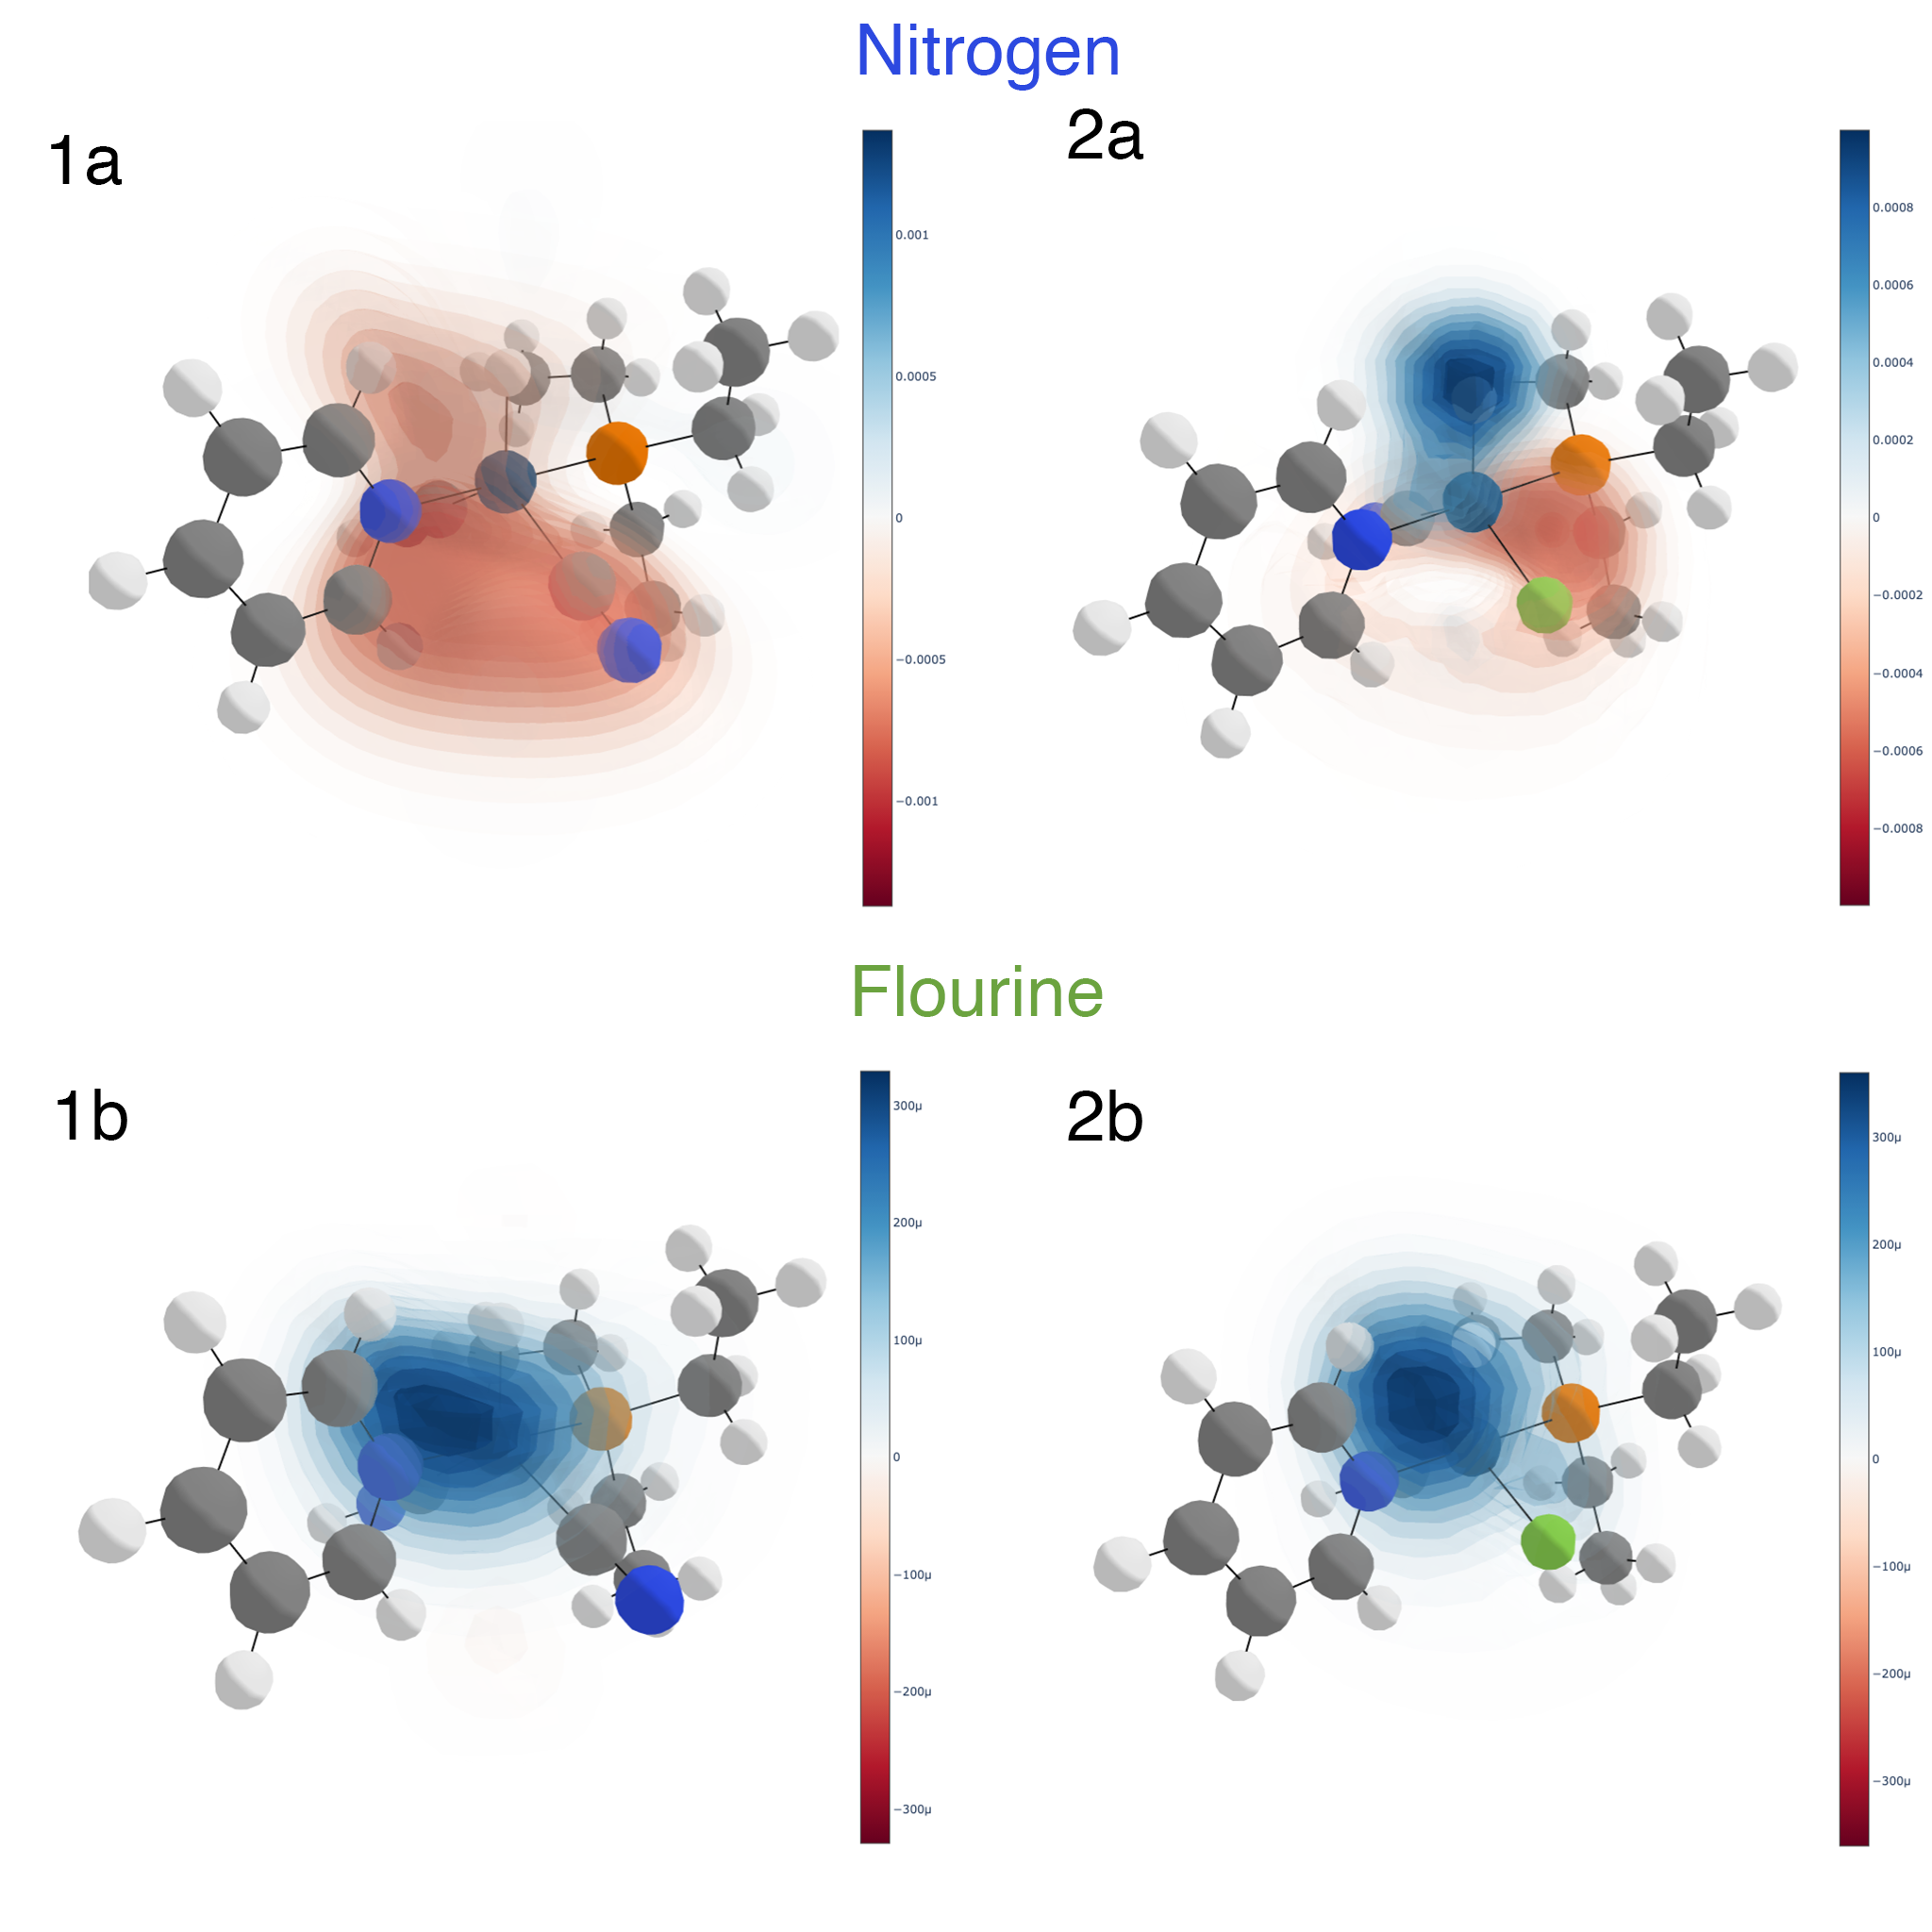
\includegraphics[width=0.9\textwidth]{figures/evaluation/GradientComp.png}
  \caption[Comparison of local gradients]{
      Gradient of a model trained on features with $n_{max}=8, l_{max}=4$ translated into 3D space.
      The element on the left has an activation barrier of $3.6 kcal/mol$, while the element on that right
      has an activation barrier of $18.0 kcal/mol$.
      The chemical structures of the molecules are identical except for the nitrogen(blue) arm of the element
      on the left being exchanged for a fluorine(green) arm for the molecule on the right.
      On the top, the gradient for nitrogen is plotted. On the bottom, the gradient for fluorine is plotted.
      More angles for plot 1a can be found in Figure~\ref{fig:gradient-sides}.
   }
  \label{fig:snap-gradient}
\end{figure}

Here the encoding limitations introduced earlier are encountered.
For some atoms, the encoding seems to work as expected, producing regions of negative gradient density where
an increase in the activation barrier is expected, for others the distribution is not precise enough for detailed analysis.
Looking at Figure~\ref{fig:snap-gradient}, an area of negative density for the nitrogen plot 1a of element 1 can be observed.
The negativity is relativity strong in comparison with the gradient density for other elements.
This indicates that decreasing the amount of nitrogen atoms should increase the activation barrier.
This is confirmed by the data.
When exchanging one nitrogen atom for fluorine, the activation barrier increases from $3.6 kcal/mol$ to $18.0kcal/mol$.
However, when looking at the other plots, the density plot becomes less clear.
Since the addition of the fluorine atom increased the activation barrier, the expectation is that a region of strong positive
density is indicated around the fluorine atom.
While there is a region of positive density in the plot 2b, it is way off from the fluorine atom.
This would indicate adding fluorine in this region will further increase the barrier.
However adding more fluorine atoms in this region is chemically impossible. %TODO: Is it?
\\

It remains unclear what the proper interpretation of the 3D gradient density should be.
While there could be some correlation between the gradient and the actual regions where density has to be added or
removed to alter the activation barrier, differentiating between actual insight of the chemical properties and artifacts 
of the mapping between feature space and activation barrier seems challenging.

In general, the detail of the encoding does not seem high enough for localized spacial interpretation of the gradient.
Possible solutions to the resolution problem could include dramatically increasing the number of coefficients used to describe a single sample.
This comes with it's own set of challenges, since the size of the features does not scale linear, but rather in $\mathcal{O}(n_{max} \cdot {l_{max}}^3)$.
The cubic scale of $l_{max}$ implies a dramatic increase in the size of the training data, increasing computation time for booth feature generation and training of the regression model.
\\

While the local encoding does not seem the be accurate enough for detailed interpretation,
when integrating over the entire density space, an insight about the global influence for each species can be gained.
The output looks similar to what was achieved with SHAP values, but in this case insight on how changing the density for a certain species will affect the activation barrier should be gained.
This means a high density of one species should indicate that adding more density of this species will increase the barrier.
Similarly, a low density should indicate indicate that adding more density for this species will decreased the barrier. %TODO: So rum richtig??

For easier computation, instead of an integration the sum over a grid will be computed: 

$$ \rho_\nabla^Z \sim \sum_{\mathbb{R}^3} \rho_\nabla^Z $$

When looking at the integration over $\rho^Z_\nabla$, the plot is heavily dominated by hydrogen and carbon
in many cases.
Since hydrogen and carbon are used in a variety of different ligands, the interpretability
these elements is low.
For other elements, the gradient density might be a better indication 


\begin{figure}[!htb]
  \minipage{0.5\textwidth}
    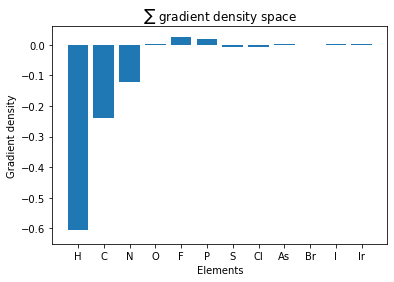
\includegraphics[width=1.0\textwidth]{figures/evaluation/elem2-GRAD.png}
  \endminipage\hfill
  \minipage{0.5\textwidth}
    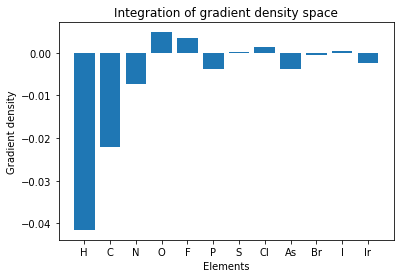
\includegraphics[width=1.0\textwidth]{figures/evaluation/elem1-GRAD.png}
  \endminipage\hfill
  \caption[Comparison of summed gradients]{
    Comparison of the gradient for molecule 1 (left) and 2 (right) for different species of atoms.
  }
  \label{fig:snap_global_gradient}

\end{figure}


It is unclear if the the chemical interpretation here should be that hydrogen and carbon play a bigger role in the activation
barrier than what was expected, or if this is an artifact of the neural network, and does not actually translate back into 
the physical world.

For other elements, the gradient behaves more like what is expected.
Looking at the nitrogen density for element 1, nitrogen has a strong negative density \ref{fig:snap_global_gradient}.
This would indicate that decreasing the amount of nitrogen in the element should increase the activation barrier.
Looking at the second element, further increasing the fluorine density should further increase the activation barrier.
Both are consistent with the calculated barriers.

For other elements, the interpretation of the gradient becomes less clear.
In some cases, the gradient does not seem to correspond to the intuition about a molecule.
The gradient also greatly varies between models trained on different $n_{max}$ and $l_{max}$ Figure~\ref{fig:snap-gradient-model}.

\begin{figure}
  \centering
  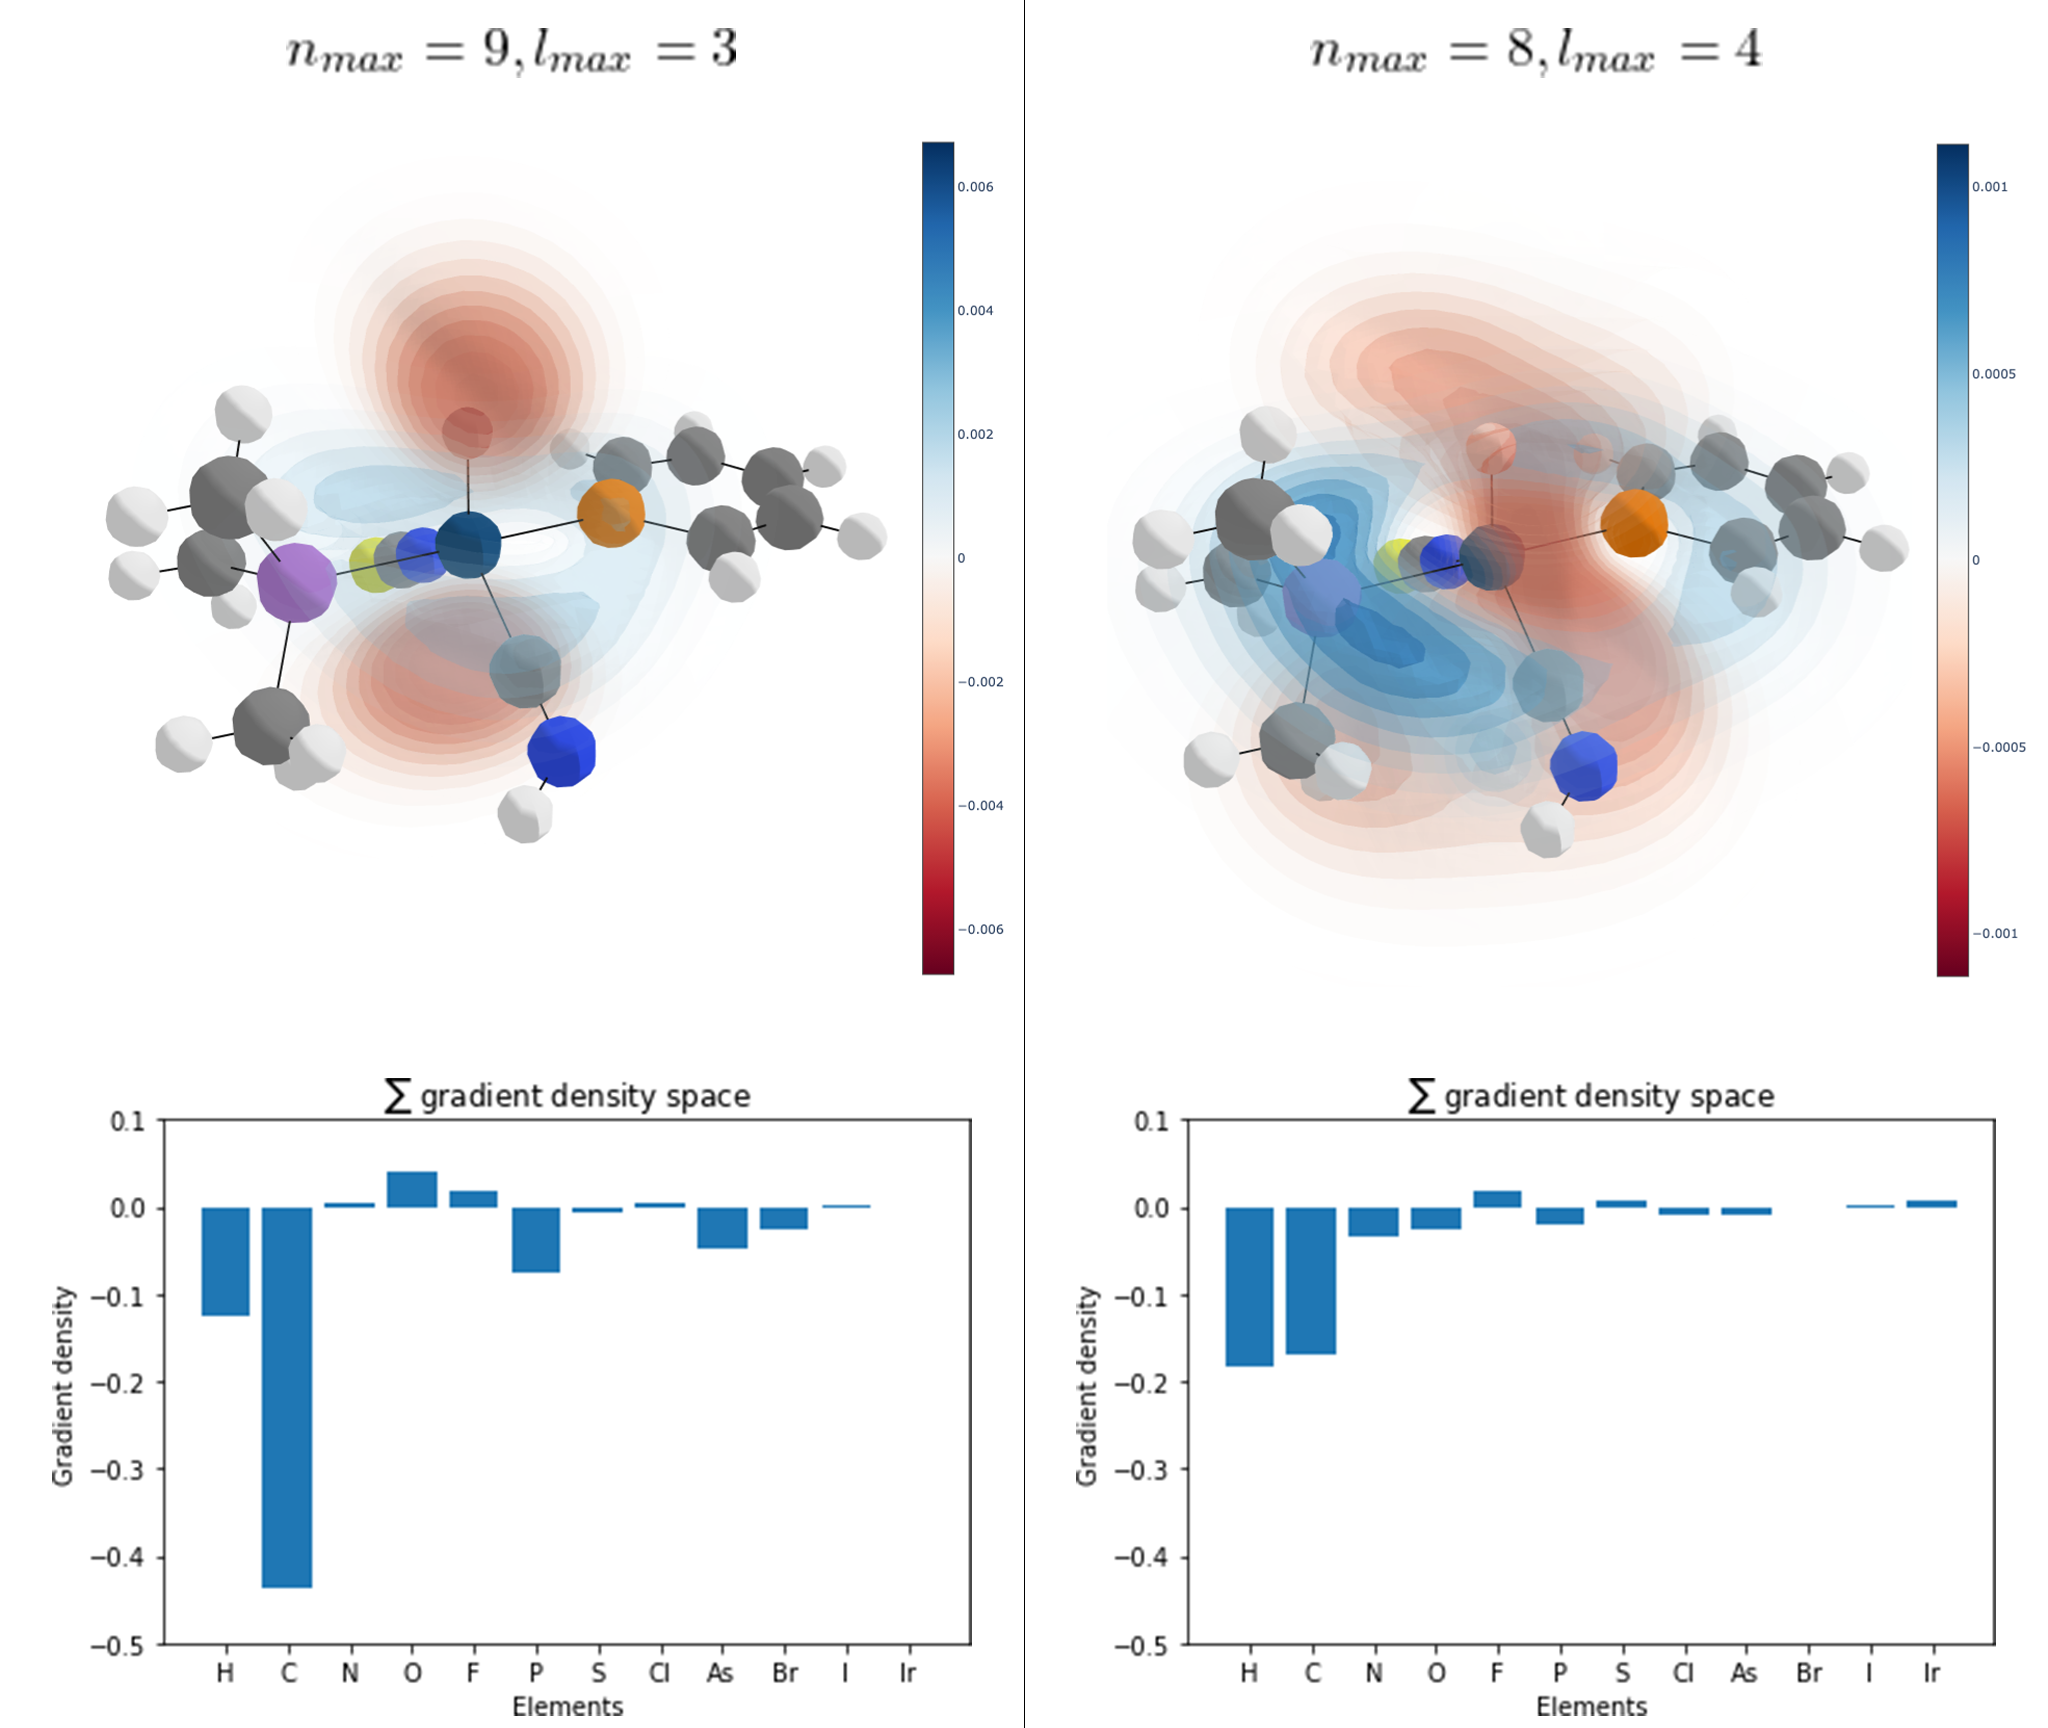
\includegraphics[width=0.9\textwidth]{figures/evaluation/Gradient-model-comp.png}
  \caption[Comparison of gradients between different models]{
      Gradient for nitrogen for the same element on 2 different models.
      The model on the left was trained on $n_{max} = 9, l_{max}=3$ while the model on the right was trained on 
      $n_{max}=8, l_{max}=4$. 
      While there are some similarities in the 3D density plot, the integration over the entire density space 
      seems to vastly differ.
   }
  \label{fig:snap-gradient-model}
\end{figure}


All these uncertainties make a general conclusion about the relevance of the gradient difficult.
While there seems to be some correlation between what is expected from the gradient and what 
the data suggests, in many cases the data seems to be unclear or contradict what the chemical intuition would be.

To use the gradient for a better chemical understanding, the networks would have to undergo a more in depth analysis.
This could include an extended dataset or a higher resolution of the feature space.

For now, the SHAP values seem to offer a better insight in how chemical properties influence the activation barrier of a catalyst.
%% conclusion.tex
%%

%% ==================
\chapter{Conclusion}
\label{ch:conclusion}
%% ==================

Summary and outlook.

%% --------------------
%% |   Bibliography   |
%% --------------------

%% Add entry to the table of contents for the bibliography
\printbibliography[heading=bibintoc]

%% ----------------
%% |   Appendix   |
%% ----------------
\appendix
%% LaTeX2e class for student theses
%% sections/apendix.tex
%% 
%% Karlsruhe Institute of Technology
%% Institute for Program Structures and Data Organization
%% Chair for Software Design and Quality (SDQ)
%%
%% Dr.-Ing. Erik Burger
%% burger@kit.edu
%%
%% Version 1.3.5, 2020-06-26

\iflanguage{english}
{\chapter{Appendix}}    % english style
{\chapter{Anhang}}      % german style
\label{chap:appendix}


%% -------------------
%% | Example content |
%% -------------------
\section{First Appendix Section}
\label{sec:appendix:FirstSection}
		
\setcounter{figure}{0}
		
\begin{figure} [ht]
  \centering
  \caption{A figure}
  \label{fig:anotherfigure}
\end{figure}


\dots
%% ---------------------
%% | / Example content |
%% ---------------------

\end{document}
